\documentclass[8pt]{beamer}

\newif\ifplacelogo % create a new conditional
\placelogotrue % set it to true

\usetheme{Warsaw}
\usecolortheme{rose}
\usepackage{multicol}
\usepackage{epstopdf}
\usepackage[italic]{hepnames}
\usepackage{tikz}
\usepackage{listings}
\usepackage{times}
\usepackage{amsmath}
\usepackage{verbatim}
\usepackage{hyperref}
\usepackage{bbding}
\lstset{breakatwhitespace,
language=C++,
columns=fullflexible,
keepspaces,
breaklines,
tabsize=3, 
showstringspaces=false,
extendedchars=true}

% TikZ includes!!!
\usepackage{tikz}
\usetikzlibrary{backgrounds}
\usetikzlibrary{calc}
\tikzstyle{every picture}+=[remember picture]
\input{/home/oviazlo/Desktop/beamerPresentations/myReports/latexHelpScripts/tikzGrid.tex}


\begin{document}

% custom colors
\definecolor{olive}{rgb}{0.3, 0.4, .1}
\definecolor{fore}{RGB}{249,242,215}
\definecolor{back}{RGB}{51,51,51}
\definecolor{title}{RGB}{255,0,90}
\definecolor{dgreen}{rgb}{0.,0.6,0.}
\definecolor{gold}{rgb}{1.,0.84,0.}
\definecolor{JungleGreen}{cmyk}{0.99,0,0.52,0}
\definecolor{BlueGreen}{cmyk}{0.85,0,0.33,0}
\definecolor{RawSienna}{cmyk}{0,0.72,1,0.45}
\definecolor{Magenta}{cmyk}{0,1,0,0}

\definecolor{PixelColor}{RGB}{207,232,139}
\definecolor{SCTColor}{RGB}{167,166,255}
\definecolor{TRTColor}{RGB}{250,224,140}
\definecolor{grayColor}{RGB}{153,153,153}

\newcommand{\yRefPosOne}{0.0}
\newcommand{\xRefPosOne}{0.0}
\newcommand{\yRefPosTwo}{0.0}
\newcommand{\xRefPosTwo}{0.0}
\newcommand{\yRefIncrementOne}{0.0}
\newcommand{\xRefIncrementOne}{0.0}
\newcommand{\yRefIncrementTwo}{0.0}
\newcommand{\xRefIncrementTwo}{0.0}

\graphicspath{ {/home/oviazlo/Desktop/beamerPresentations/FCCee/pictures/plots_mar2/} }
\DeclareGraphicsExtensions{.eps, .pdf, .png}

\newcommand{\myBox}[2][pink] {
    \noindent\colorbox{#1}{
	\textbf{#2}
    }\par
}

% For nice block (provided by Oleh)
\tikzstyle{mybox} = [draw=red, fill=blue!1, very thick,
    rectangle, rounded corners, inner sep=5pt, inner ysep=9pt]
    
\tikzstyle{PixelBox} = [draw=PixelColor, fill=blue!1, very thick,
    rectangle, rounded corners, inner sep=5pt, inner ysep=9pt]
\tikzstyle{SCTBox} = [draw=SCTColor, fill=blue!1, very thick,
    rectangle, rounded corners, inner sep=5pt, inner ysep=9pt]
\tikzstyle{TRTBox} = [draw=TRTColor, fill=blue!1, very thick,
    rectangle, rounded corners, inner sep=5pt, inner ysep=9pt]

% poster advertisement
\newcommand{\myCenterBox}[2][pink] {
   {\centering
    \noindent\colorbox{#1}{
	\textbf{#2}
    }\par
  }
}

\newcommand{\mySmallCenterBox}[2][pink] {
   {\centering
    \noindent\colorbox{#1}{
	\textbf{{\small #2}}
    }\par
  }
}

\newcommand{\myVerySmallCenterBox}[2][pink] {
   {\centering
    \noindent\colorbox{#1}{
	\textbf{{\scriptsize #2}}
    }\par
  }
}

\newcommand{\backupbegin}{
   \newcounter{finalframe}
   \setcounter{finalframe}{\value{framenumber}}
}
\newcommand{\backupend}{
   \setcounter{framenumber}{\value{finalframe}}
}

\newcommand{\myNode}{\tikz[baseline,inner sep=1pt] \node[anchor=base]}

\definecolor{light-gray}{gray}{0.95}
% poster advertisement


\title[ Electron PID Efficiency with FCC-ee Detector \hspace{12.5em}\insertframenumber/
\inserttotalframenumber]{ Electron PID Efficiency with FCC-ee Detector }


	\author[Oleksandr Viazlo]{Oleksandr Viazlo \\ 
% 	{\small ???}
	}
	\institute{\small CERN\\} 
	
       
	\date{24 January 2018}

% 	\logo{ \ifplacelogo \includegraphics[height=1.8cm]{./ID_week2/lund_uni-logo_s.pdf} \hspace{0.4cm} \fi}

	
%    	\frame{\titlepage}

   	

\placelogofalse

%*****************************************************************************
\begin{frame}{\large \large Events with 2 photons reconstructed}
 
\renewcommand{\yRefPosOne}{0}
\renewcommand{\xRefPosOne}{5.3}
\renewcommand{\xRefIncrementOne}{5.5}
\begin{tikzpicture}[overlay]

   \node[inner sep=0pt] (tmp) at (\xRefPosOne-3,\yRefPosOne+1.5)
    {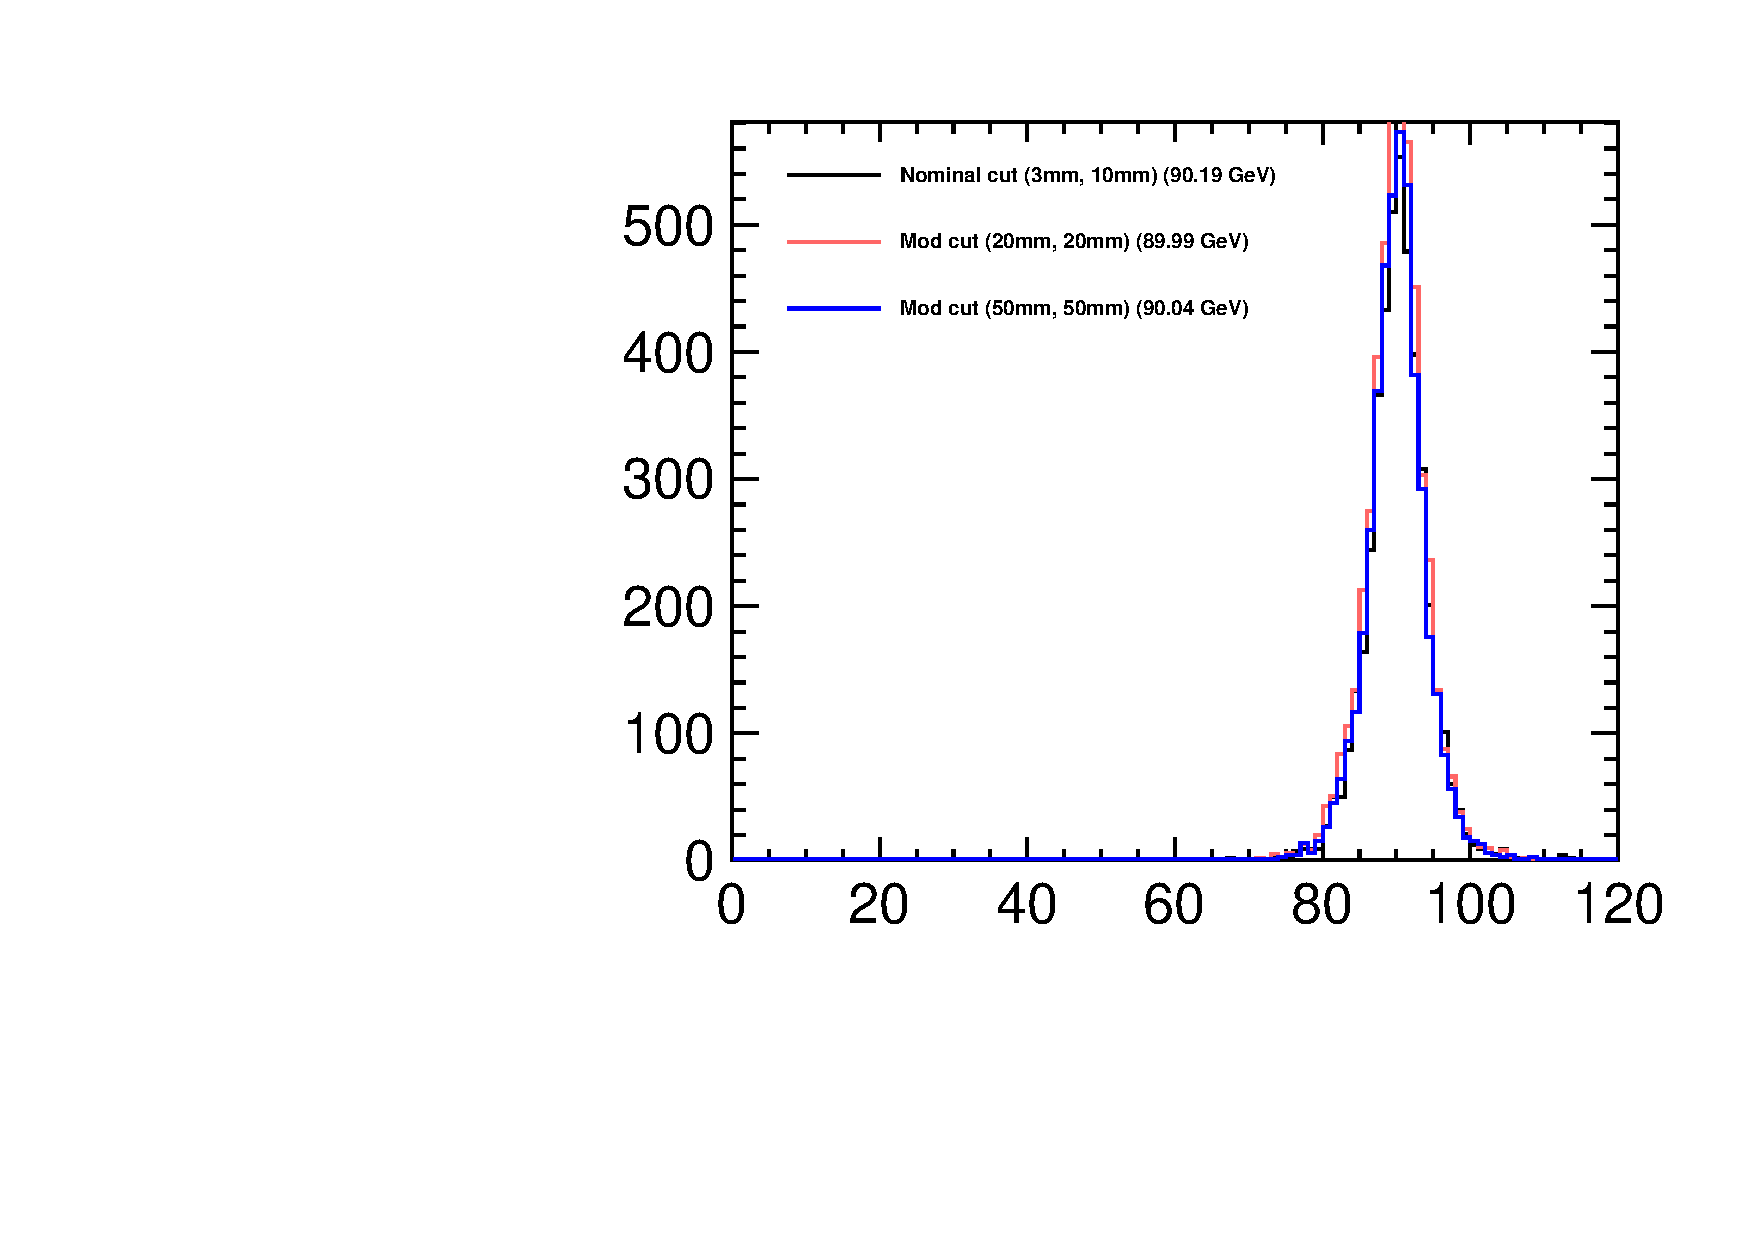
\includegraphics[width=5cm]{TrackClusterDistanceCut_totalEnergy_Zuds91.pdf}};
 
   \node[inner sep=0pt] (tmp) at (\xRefPosOne+3,\yRefPosOne+1.5)
    {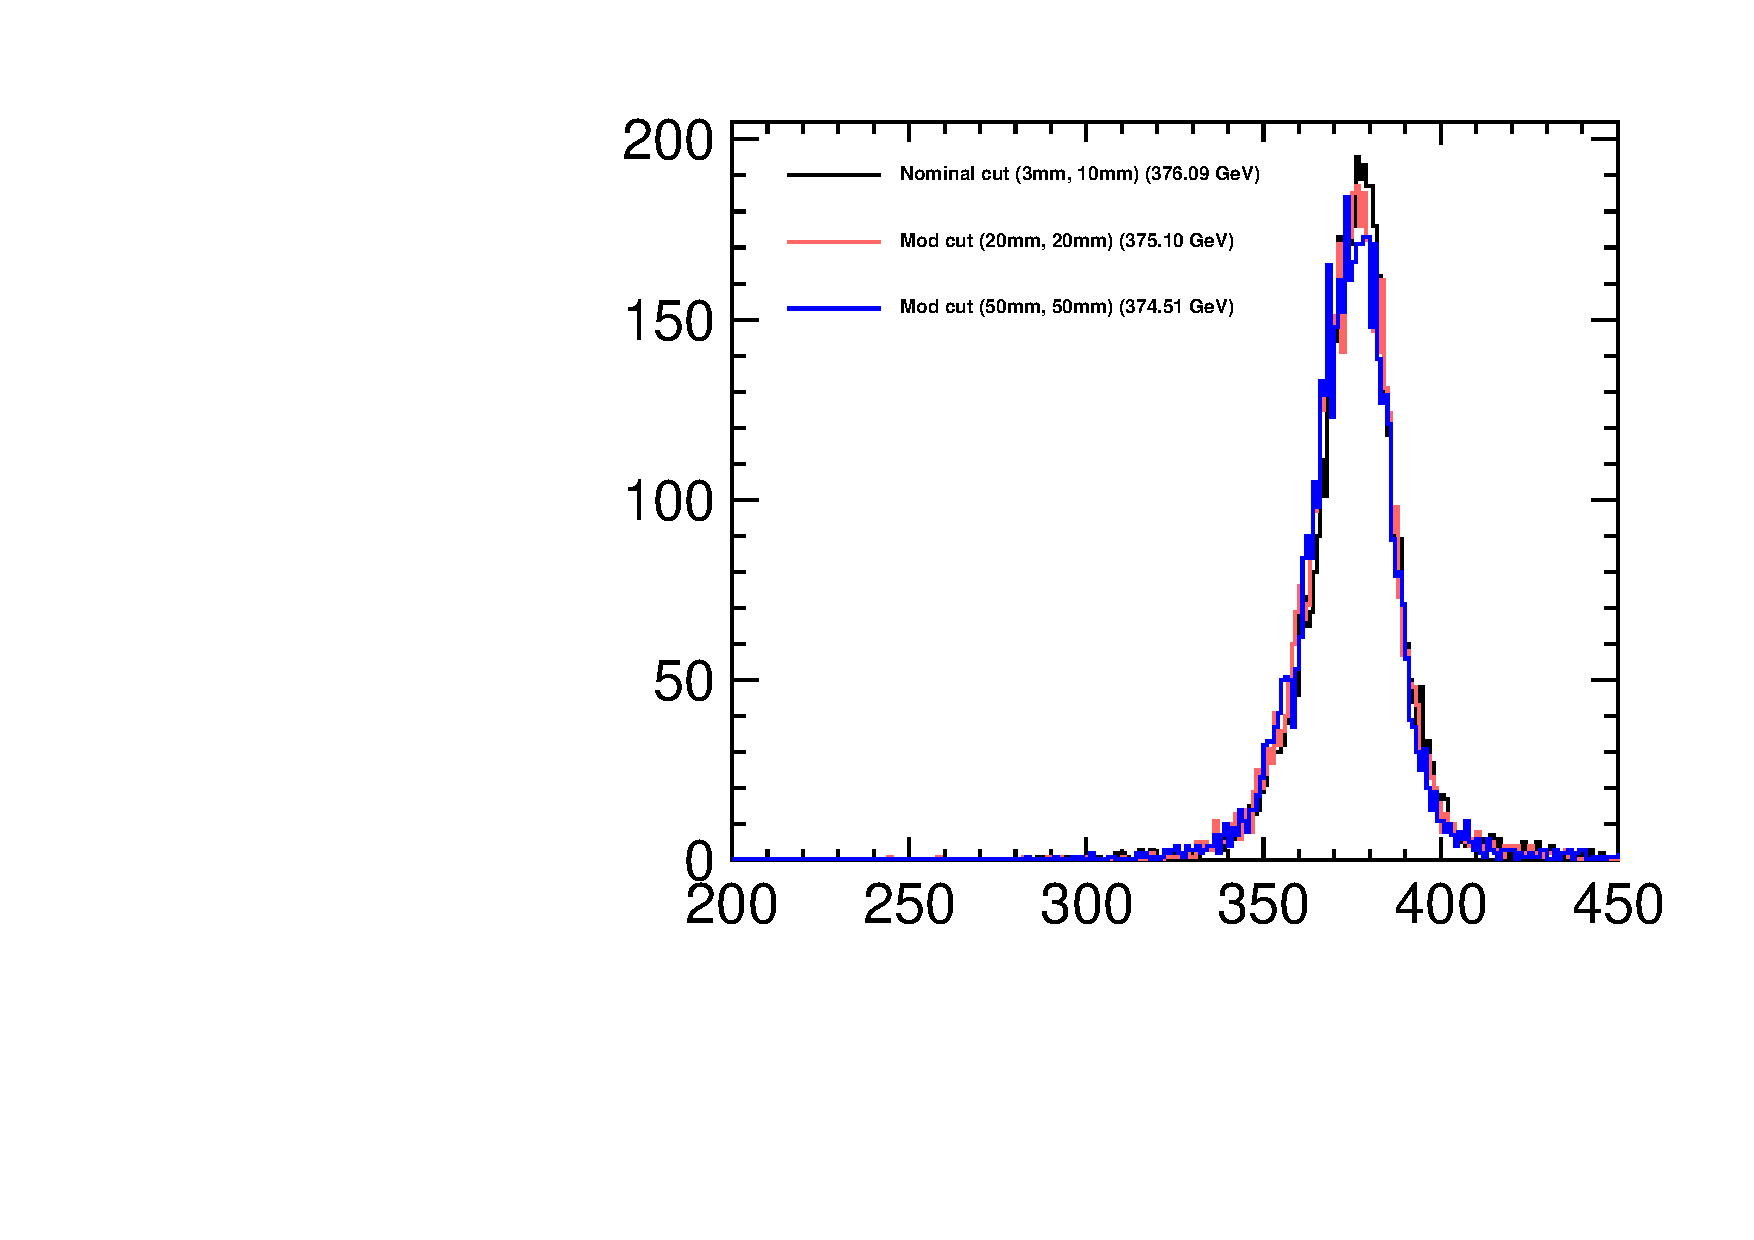
\includegraphics[width=5cm]{TrackClusterDistanceCut_totalEnergy_Zuds380.pdf}};
  
   \node[inner sep=0pt] (tmp) at (\xRefPosOne-3,\yRefPosOne-2.7)
    {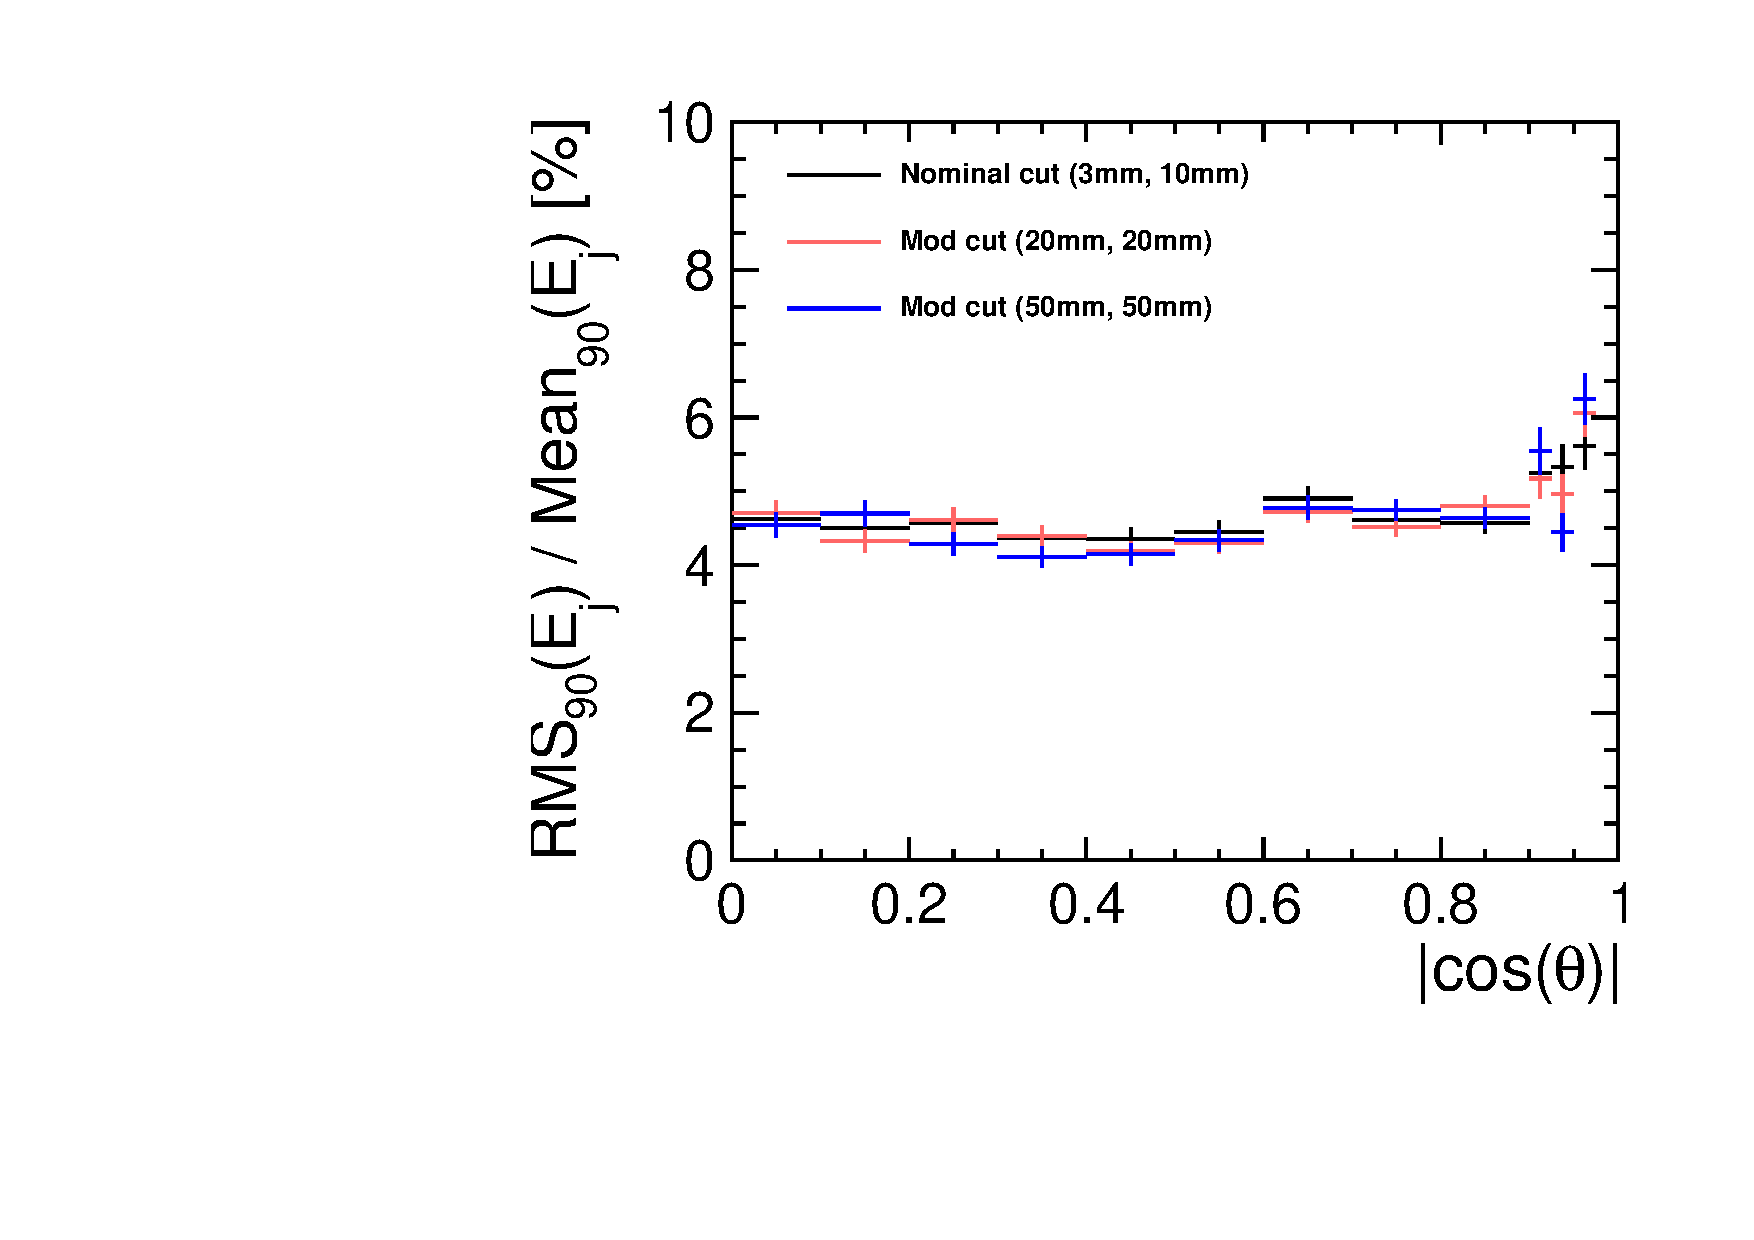
\includegraphics[width=5cm]{TrackClusterDistanceCut_resolutionVsCosTheta_Zuds91.pdf}};
 
   \node[inner sep=0pt] (tmp) at (\xRefPosOne+3,\yRefPosOne-2.7)
    {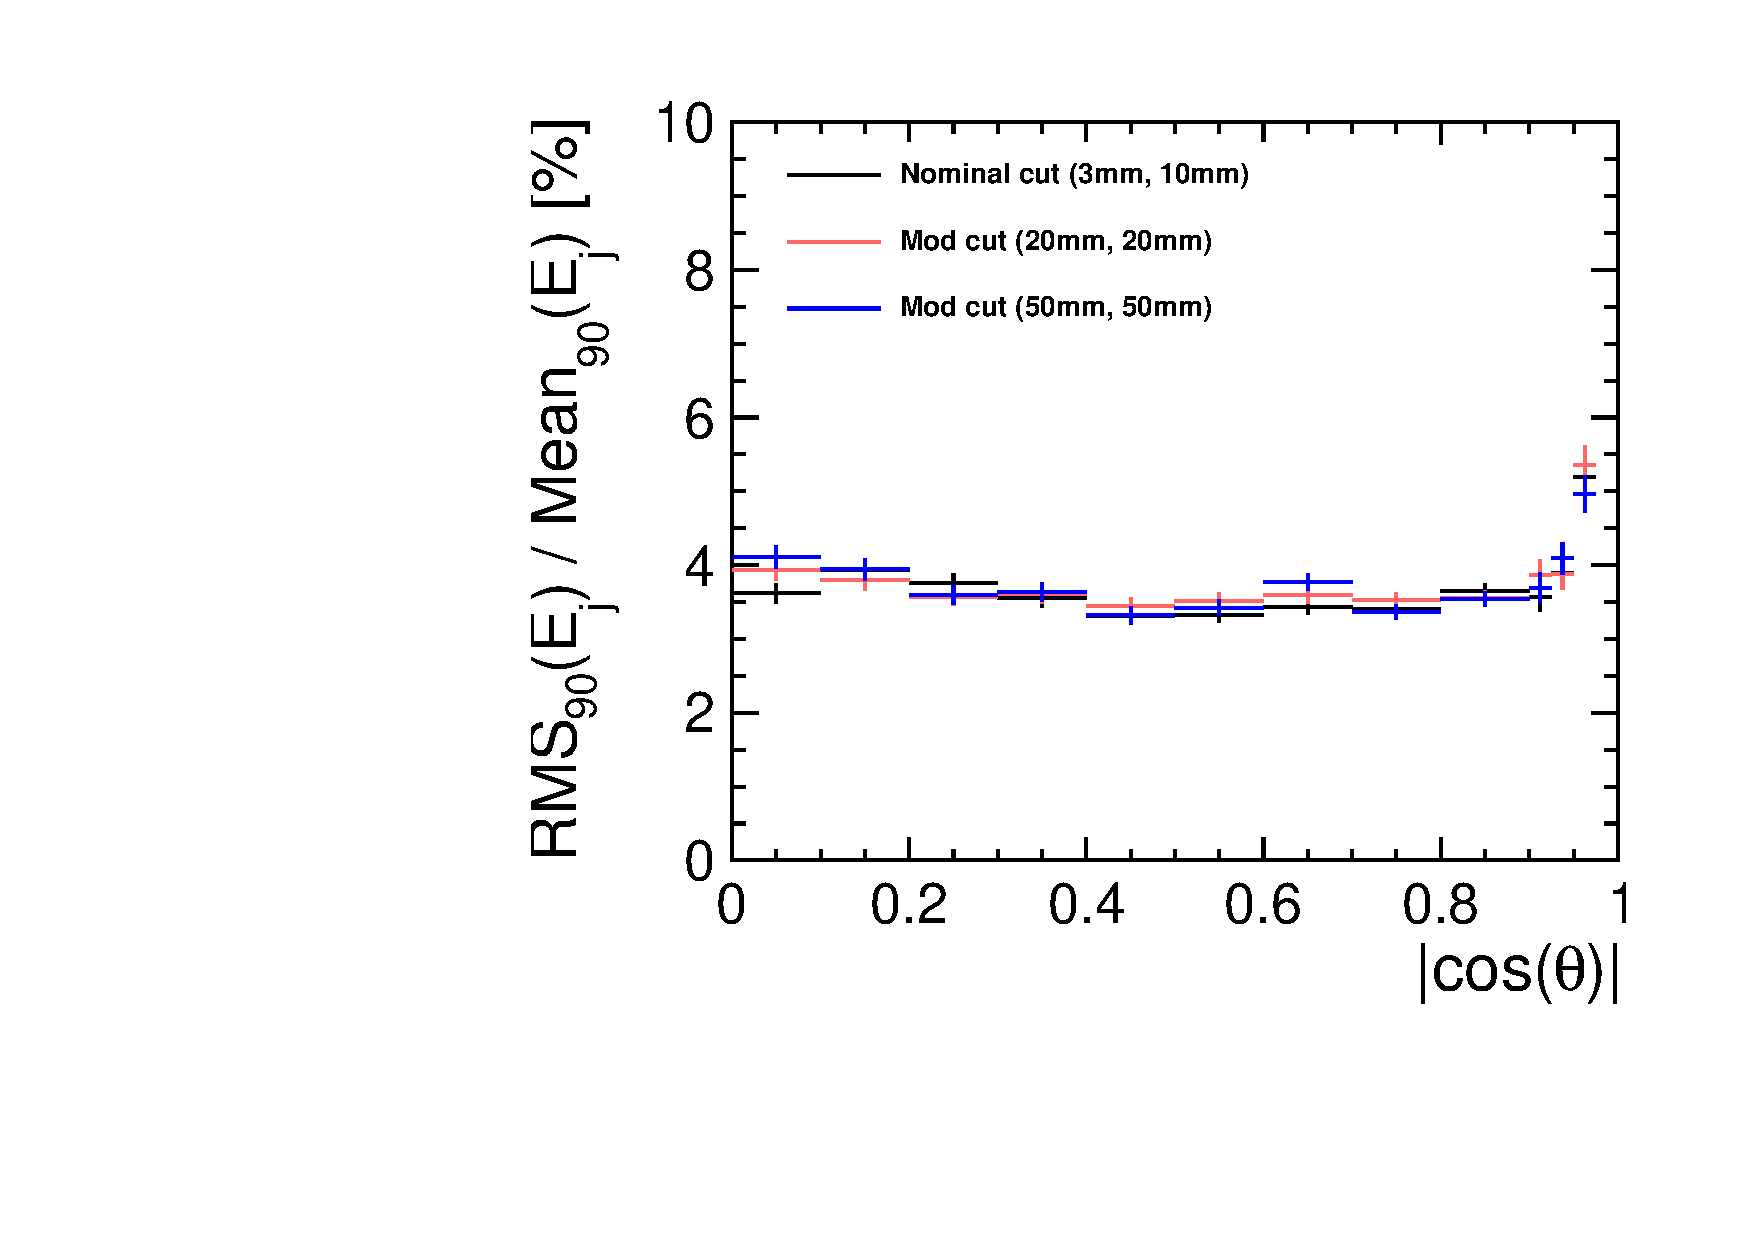
\includegraphics[width=5cm]{TrackClusterDistanceCut_resolutionVsCosTheta_Zuds380.pdf}};
  
%   \node [Box] at (\xRefPosOne-0.5,\yRefPosOne-3) (box){%
% \begin{minipage}{1\textwidth}
% 
%  \begin{itemize}
%   \item Single electron (E=10 GeV) PID efficiency for all events (left) and for events w/o bremsstrahlung (right)
%   \item Pandora doesn't reconstruct electron cluster in 10-15$\%$ of events independent of theta.
%   \item No photon misreconstruction with events w/o bremsstrahlung (right plot)
%  \end{itemize}
% \end{minipage}
% };
%   
\end{tikzpicture}
\end{frame}
%*****************************************************************************

%*****************************************************************************
\begin{frame}{\large \large Electron efficiency}
 
\renewcommand{\yRefPosOne}{0}
\renewcommand{\xRefPosOne}{5.3}
\renewcommand{\xRefIncrementOne}{5.5}
\begin{tikzpicture}[overlay]

   \node[inner sep=0pt] (tmp) at (\xRefPosOne,\yRefPosOne)
    {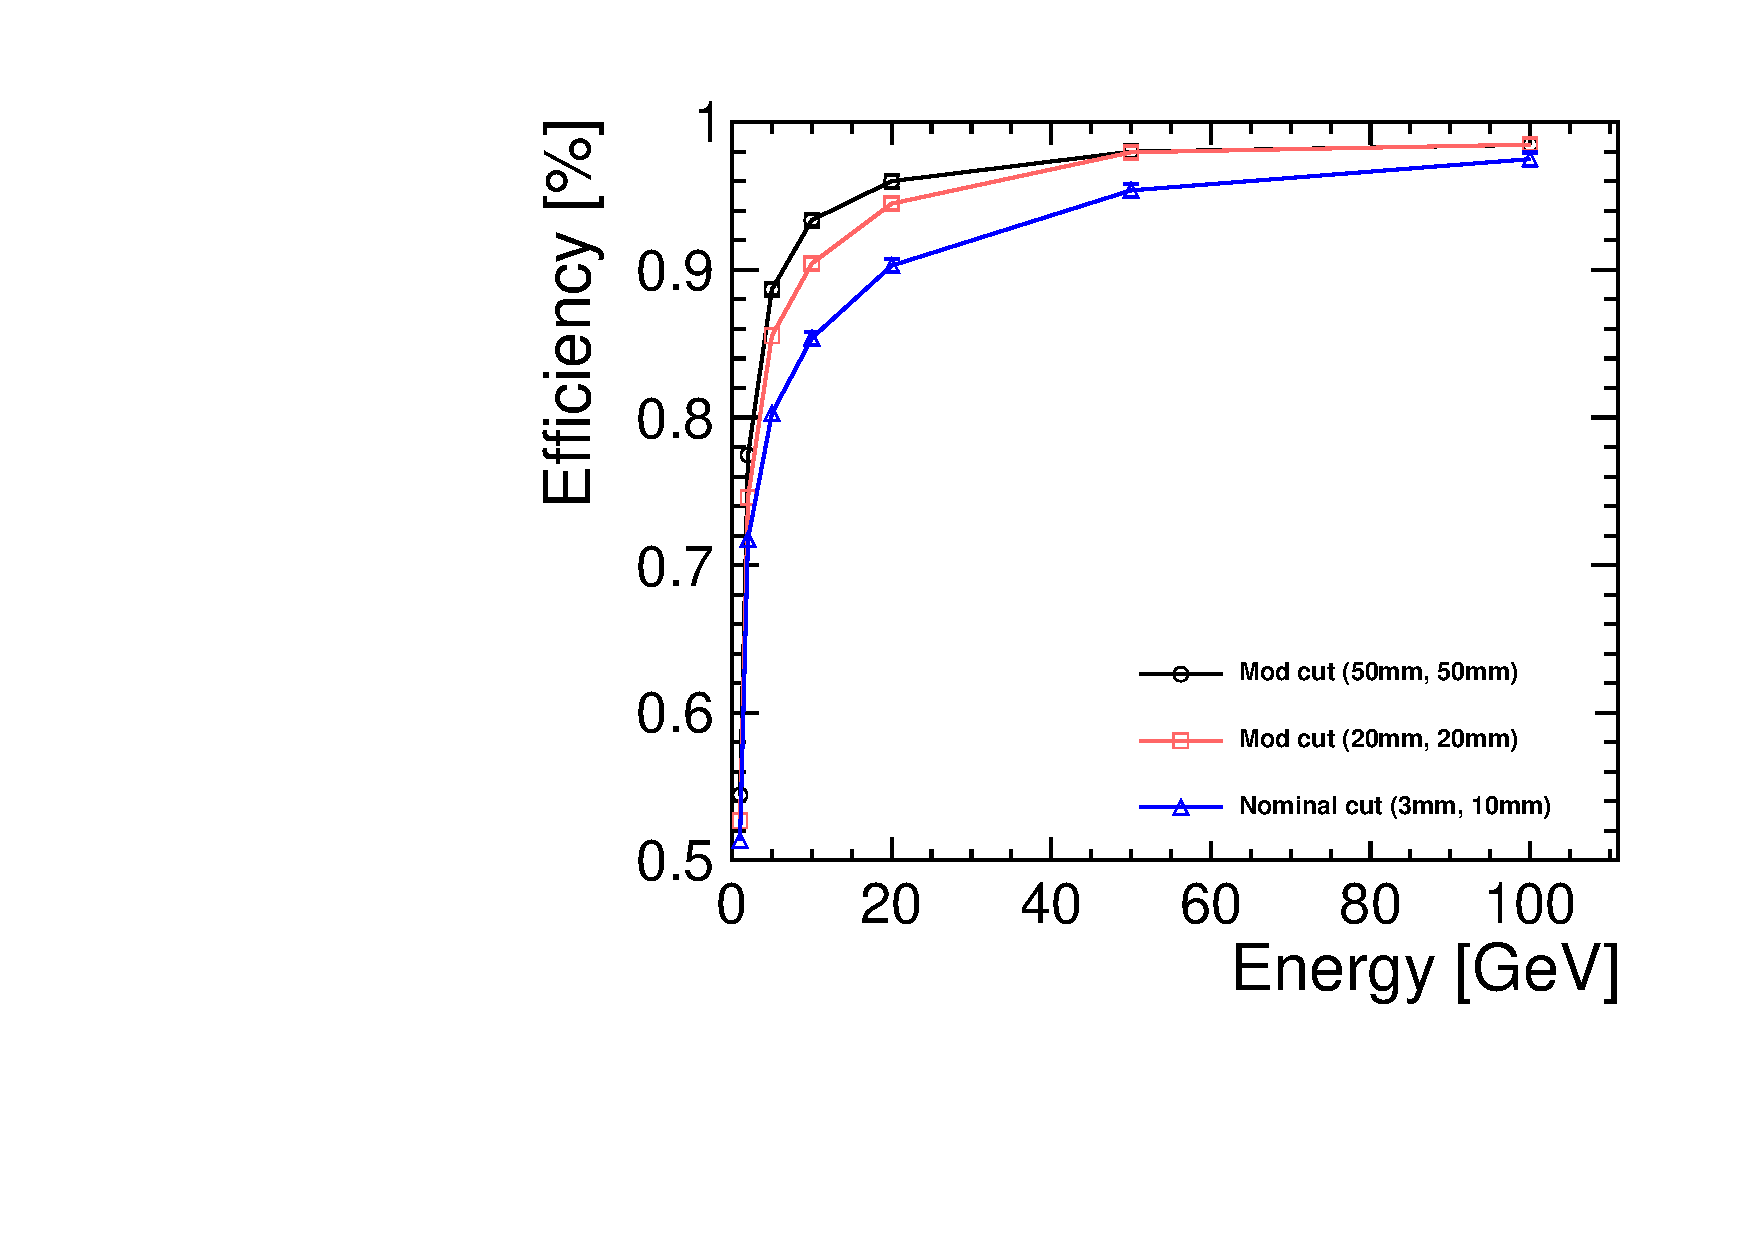
\includegraphics[width=8cm]{TrackClusterDistanceCut_effVsEnergy.pdf}}; 
 
   \node [Box] at (\xRefPosOne-0.5,\yRefPosOne-3.5) (box){%
\begin{minipage}{1\textwidth}

 \begin{itemize}
  \item PFO of electron type (no angular/energy matching)
 \end{itemize}
\end{minipage}
};
  
 
\end{tikzpicture}
\end{frame}
%*****************************************************************************

%*****************************************************************************
\begin{frame}{\large \large Total Energy: 91 GeV (top) and 380 Zuds (bottom)}
 
\renewcommand{\yRefPosOne}{0}
\renewcommand{\xRefPosOne}{5.3}
\renewcommand{\xRefIncrementOne}{5.5}
\begin{tikzpicture}[overlay]

   \node[inner sep=0pt] (tmp) at (\xRefPosOne-3,\yRefPosOne+1.5)
    {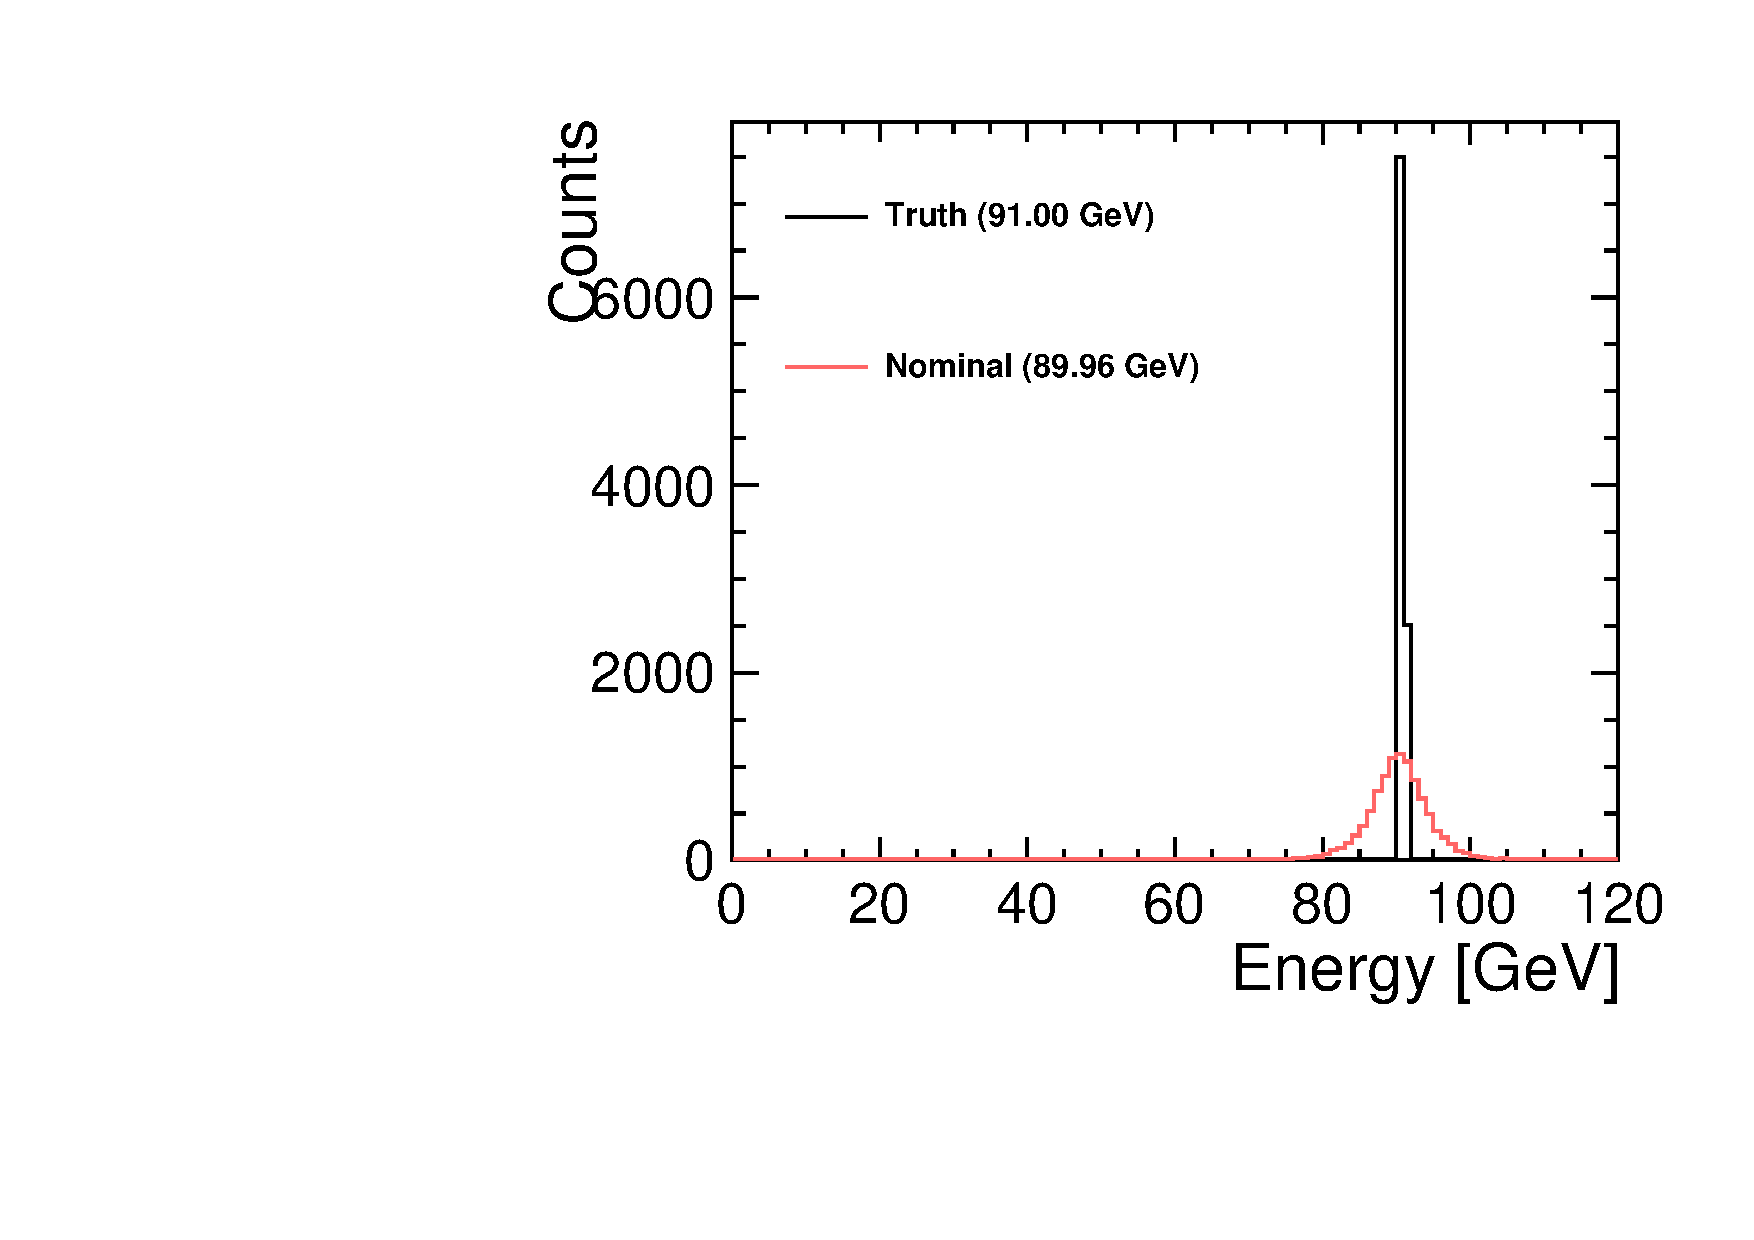
\includegraphics[width=5cm]{TrackClusterDistanceCut_Zuds91_totalEnergyRecoVsTruth.pdf}};
 
   \node[inner sep=0pt] (tmp) at (\xRefPosOne+3,\yRefPosOne+1.5)
    {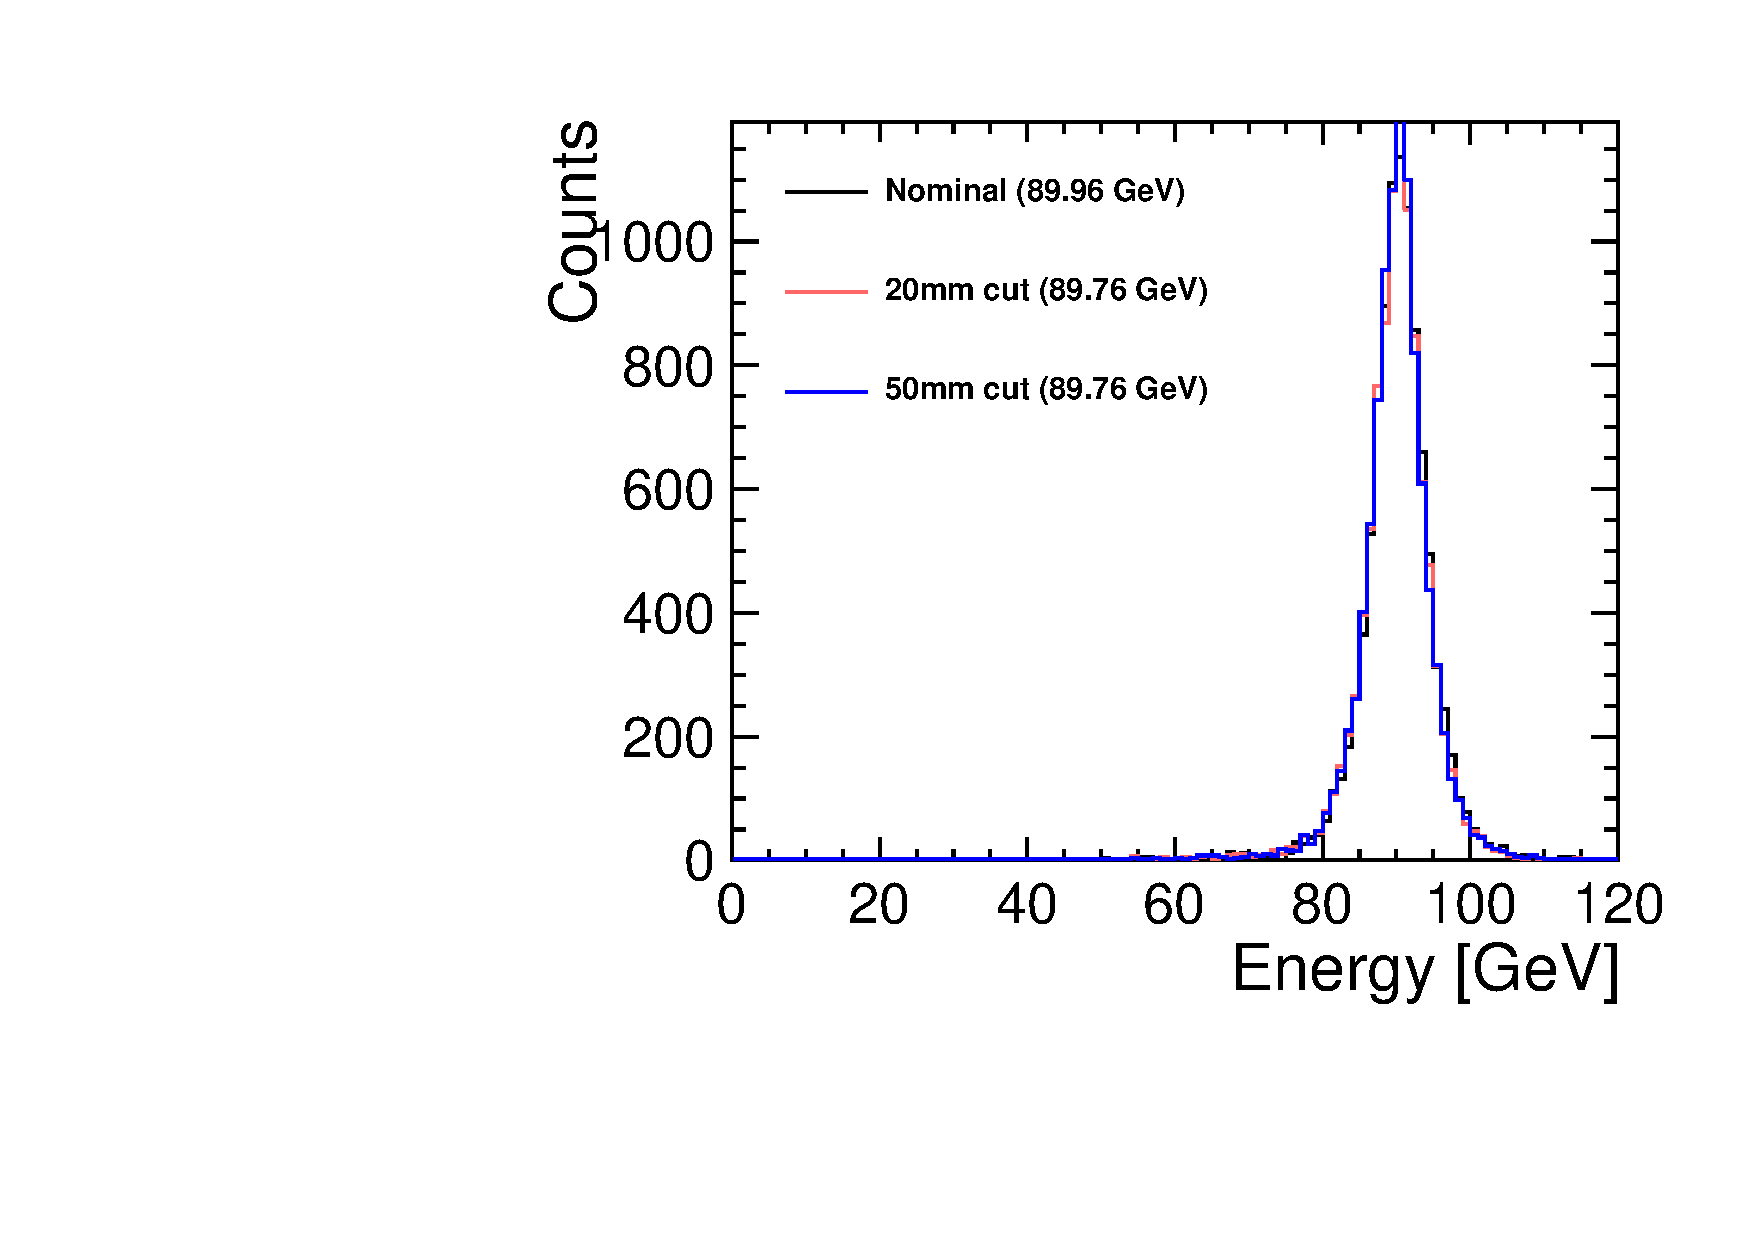
\includegraphics[width=5cm]{TrackClusterDistanceCut_Zuds91_totalRecoEnergy.pdf}};
  
   \node[inner sep=0pt] (tmp) at (\xRefPosOne-3,\yRefPosOne-2.7)
    {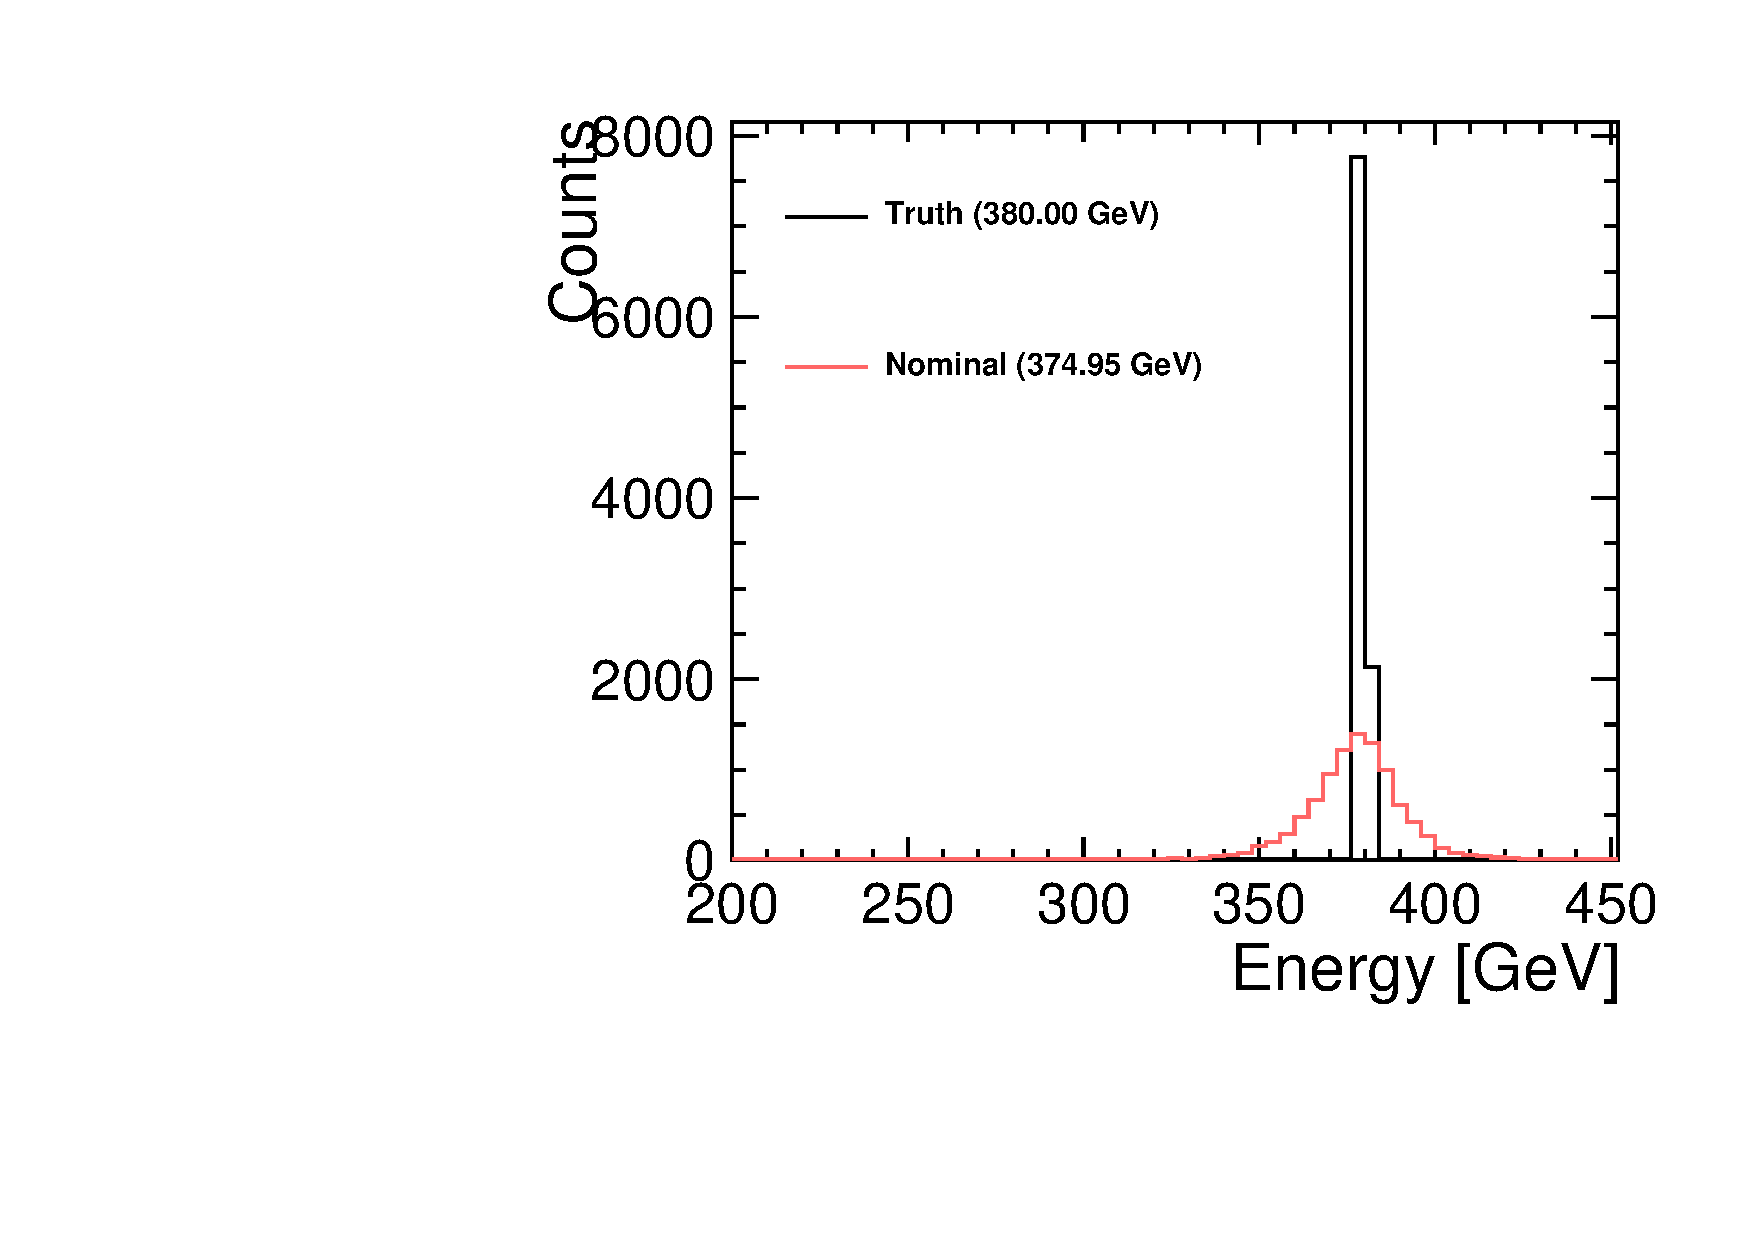
\includegraphics[width=5cm]{TrackClusterDistanceCut_Zuds380_totalEnergyRecoVsTruth.pdf}};
 
   \node[inner sep=0pt] (tmp) at (\xRefPosOne+3,\yRefPosOne-2.7)
    {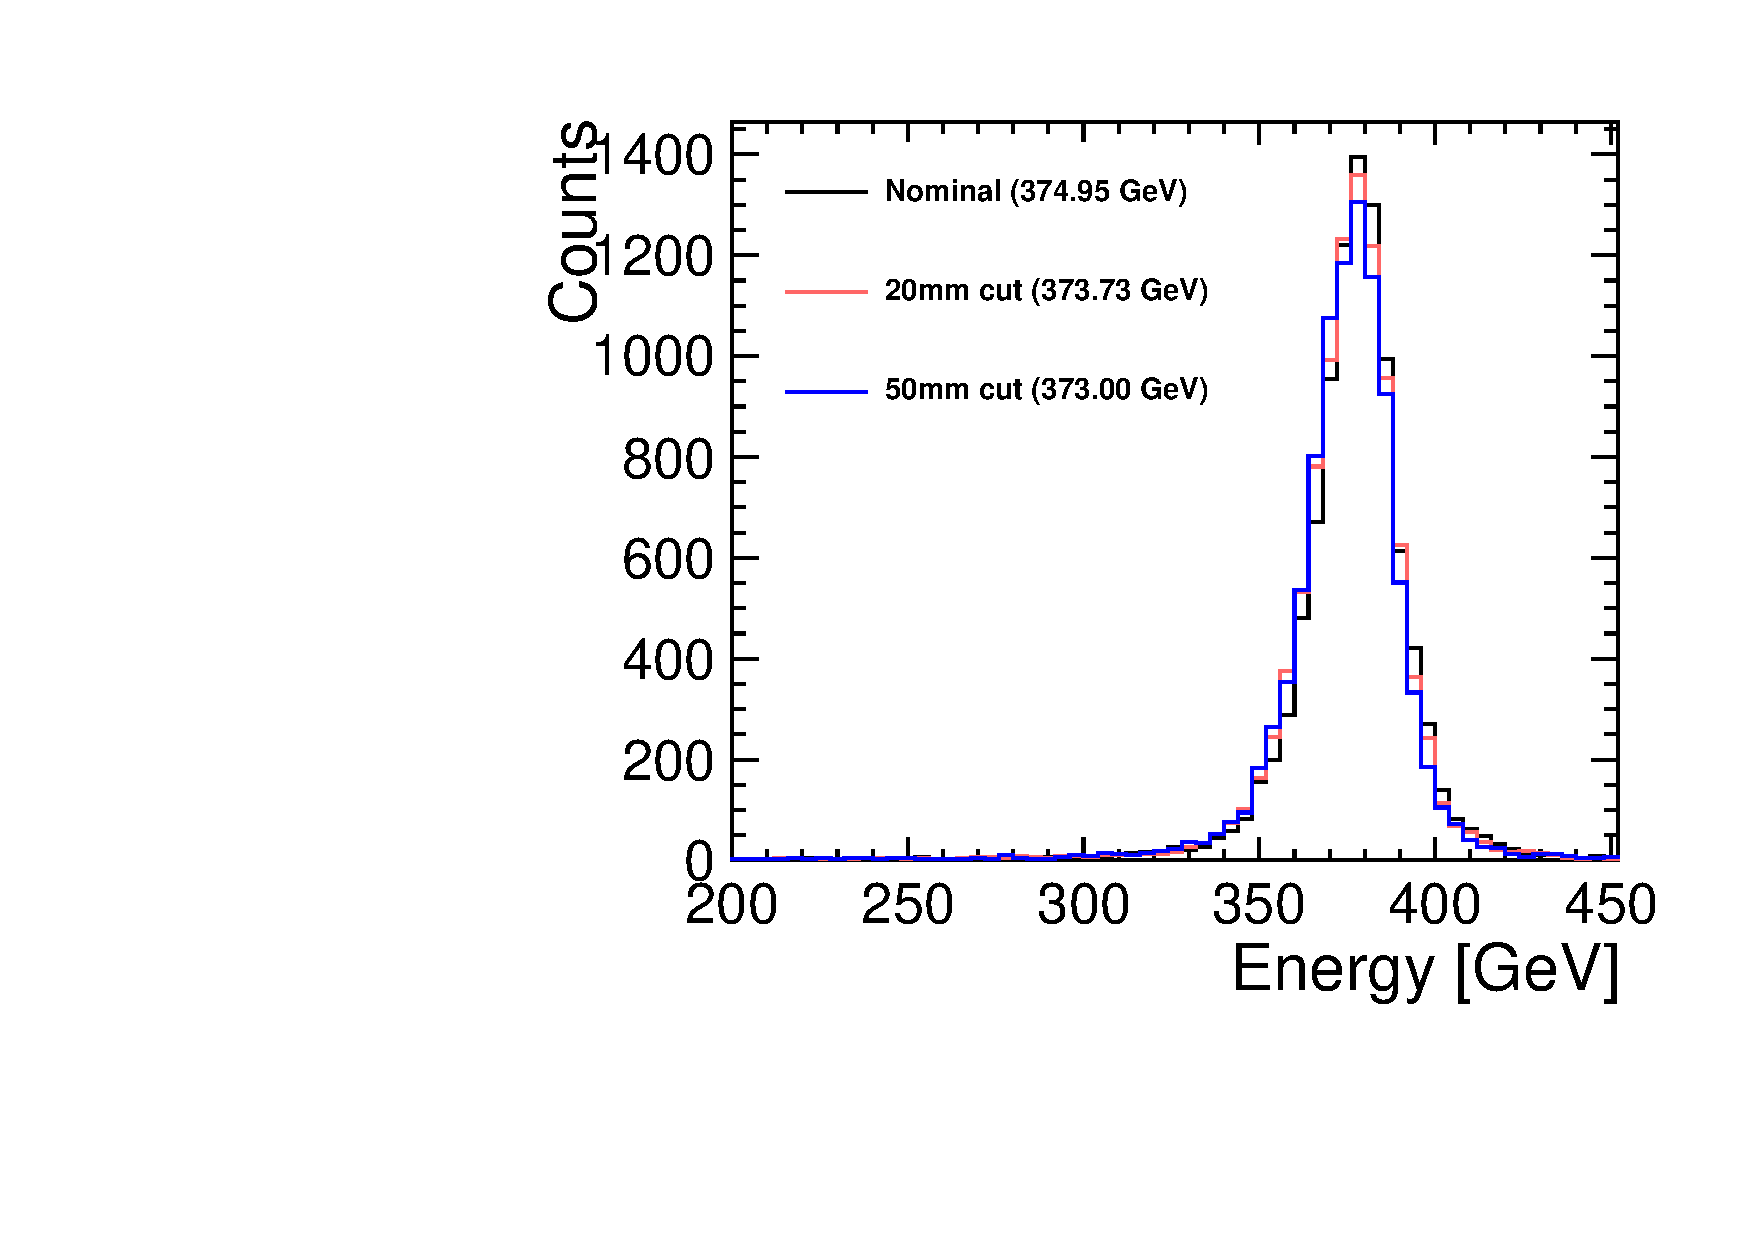
\includegraphics[width=5cm]{TrackClusterDistanceCut_Zuds380_totalRecoEnergy.pdf}};

\end{tikzpicture}
\end{frame}
%*****************************************************************************

%*****************************************************************************
\begin{frame}{\large \large Photon Energy: 91 GeV (top) and 380 Zuds (bottom)}
 
\renewcommand{\yRefPosOne}{0}
\renewcommand{\xRefPosOne}{5.3}
\renewcommand{\xRefIncrementOne}{5.5}
\begin{tikzpicture}[overlay]

   \node[inner sep=0pt] (tmp) at (\xRefPosOne-3,\yRefPosOne+1.5)
    {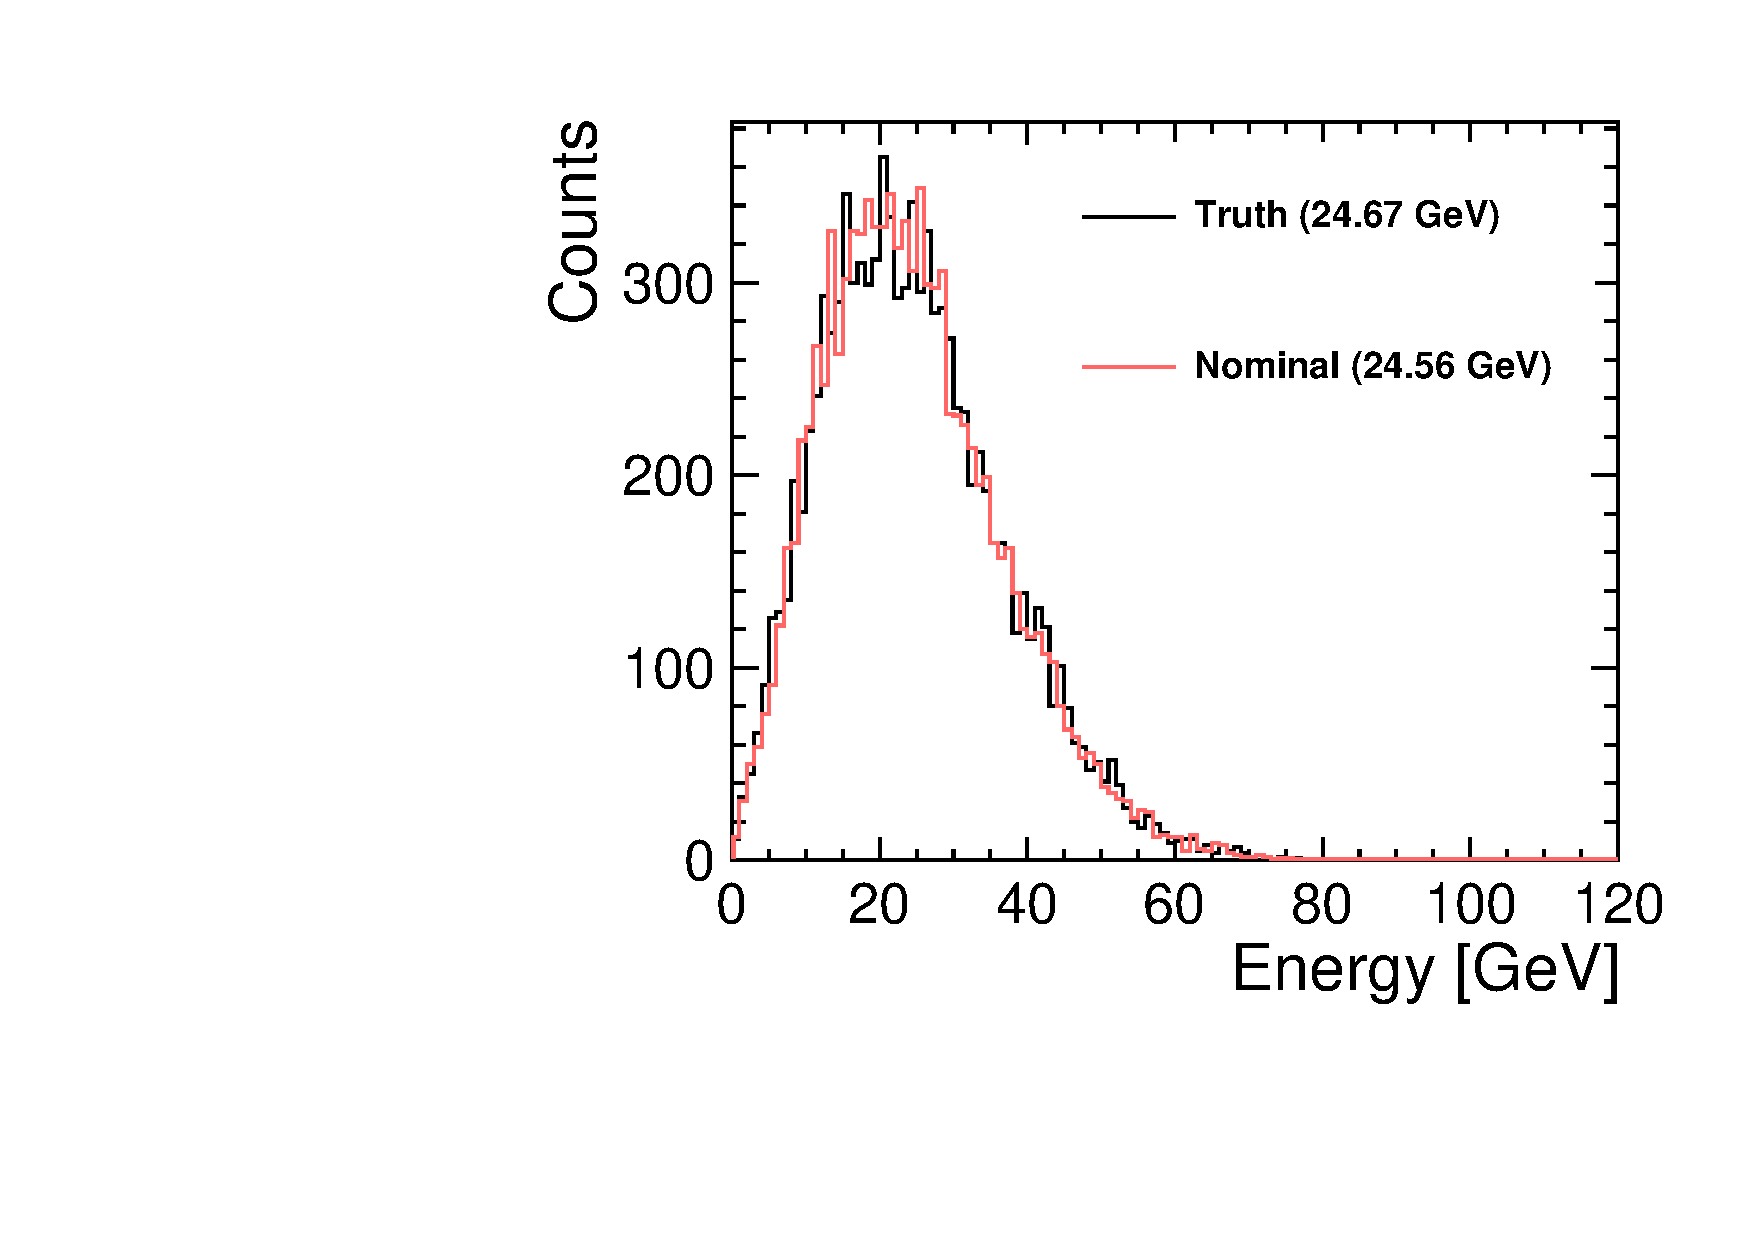
\includegraphics[width=5cm]{TrackClusterDistanceCut_Zuds91_photonEnergyRecoVsTruth.pdf}};
 
   \node[inner sep=0pt] (tmp) at (\xRefPosOne+3,\yRefPosOne+1.5)
    {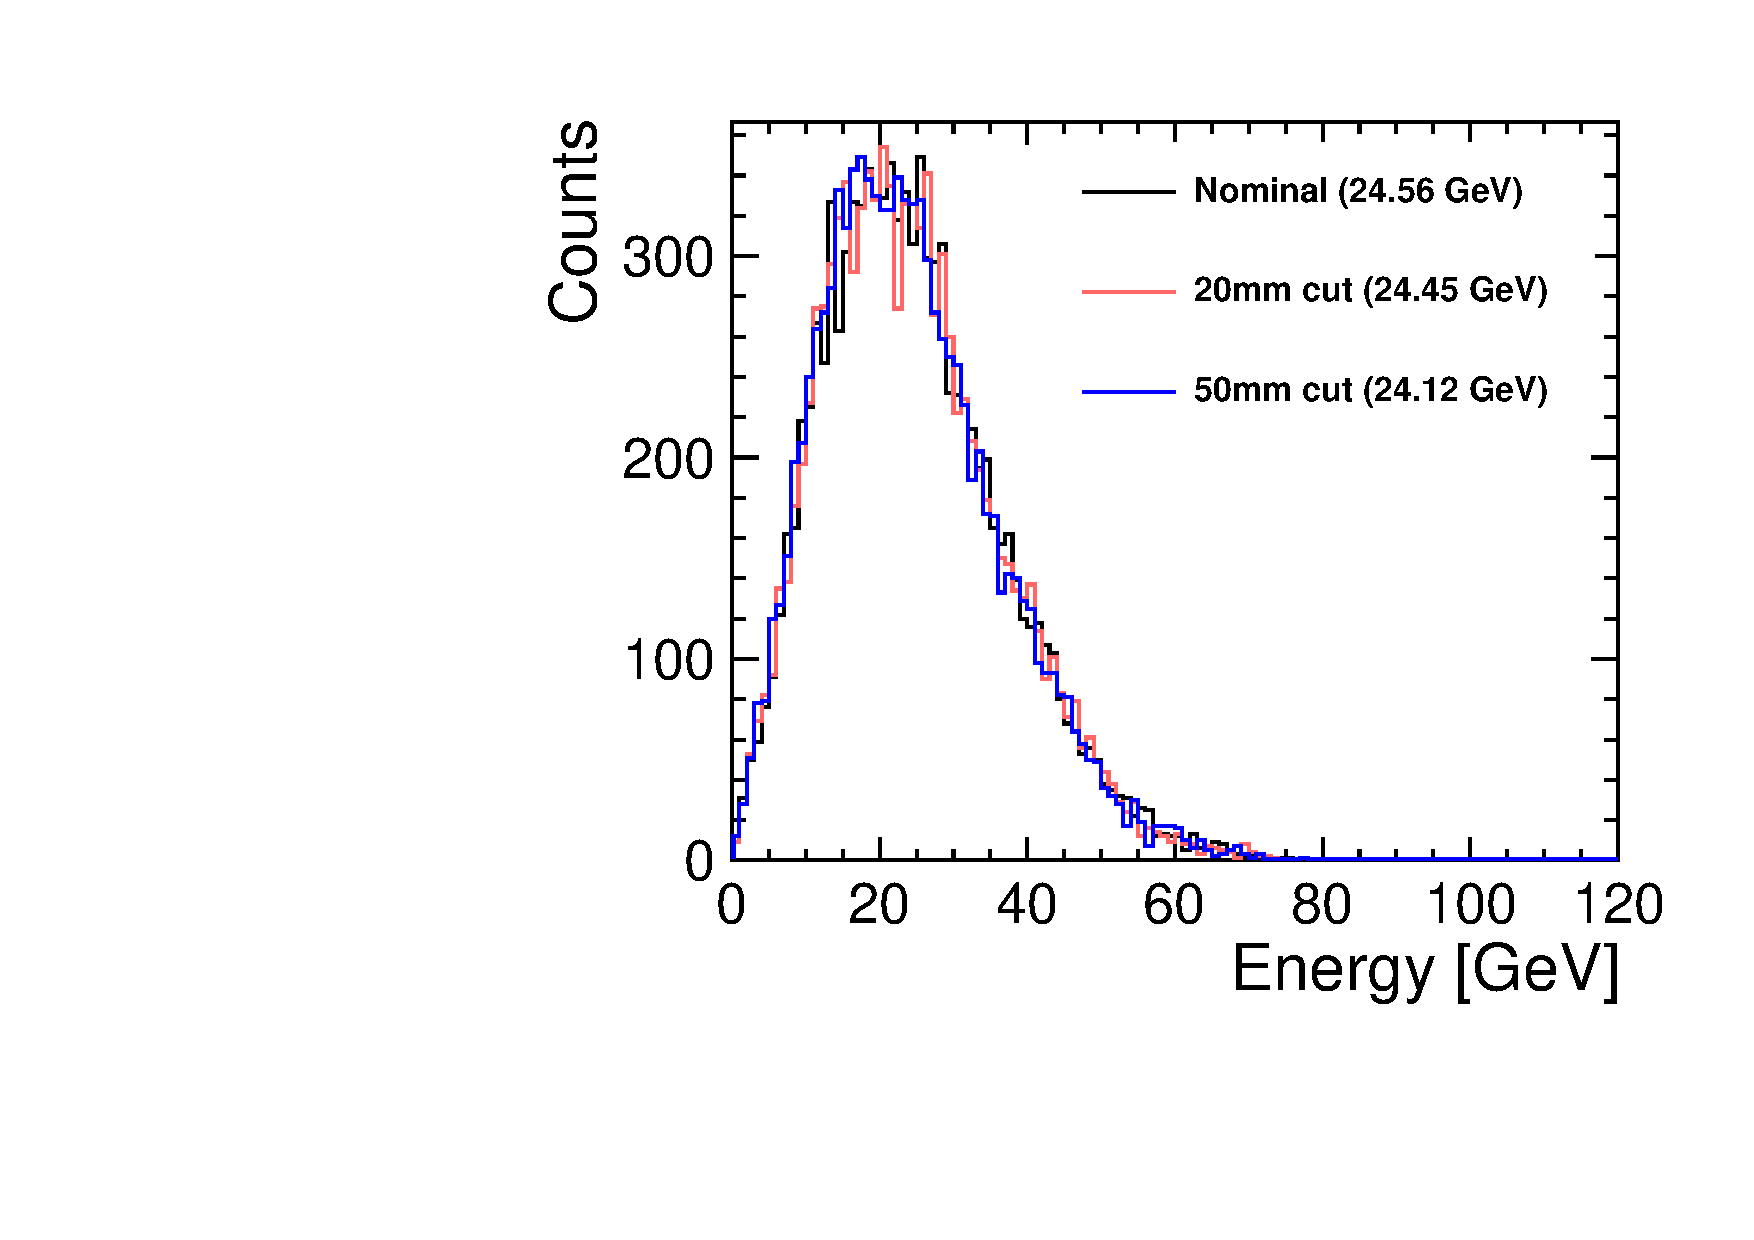
\includegraphics[width=5cm]{TrackClusterDistanceCut_Zuds91_photonRecoEnergy.pdf}};
  
   \node[inner sep=0pt] (tmp) at (\xRefPosOne-3,\yRefPosOne-2.7)
    {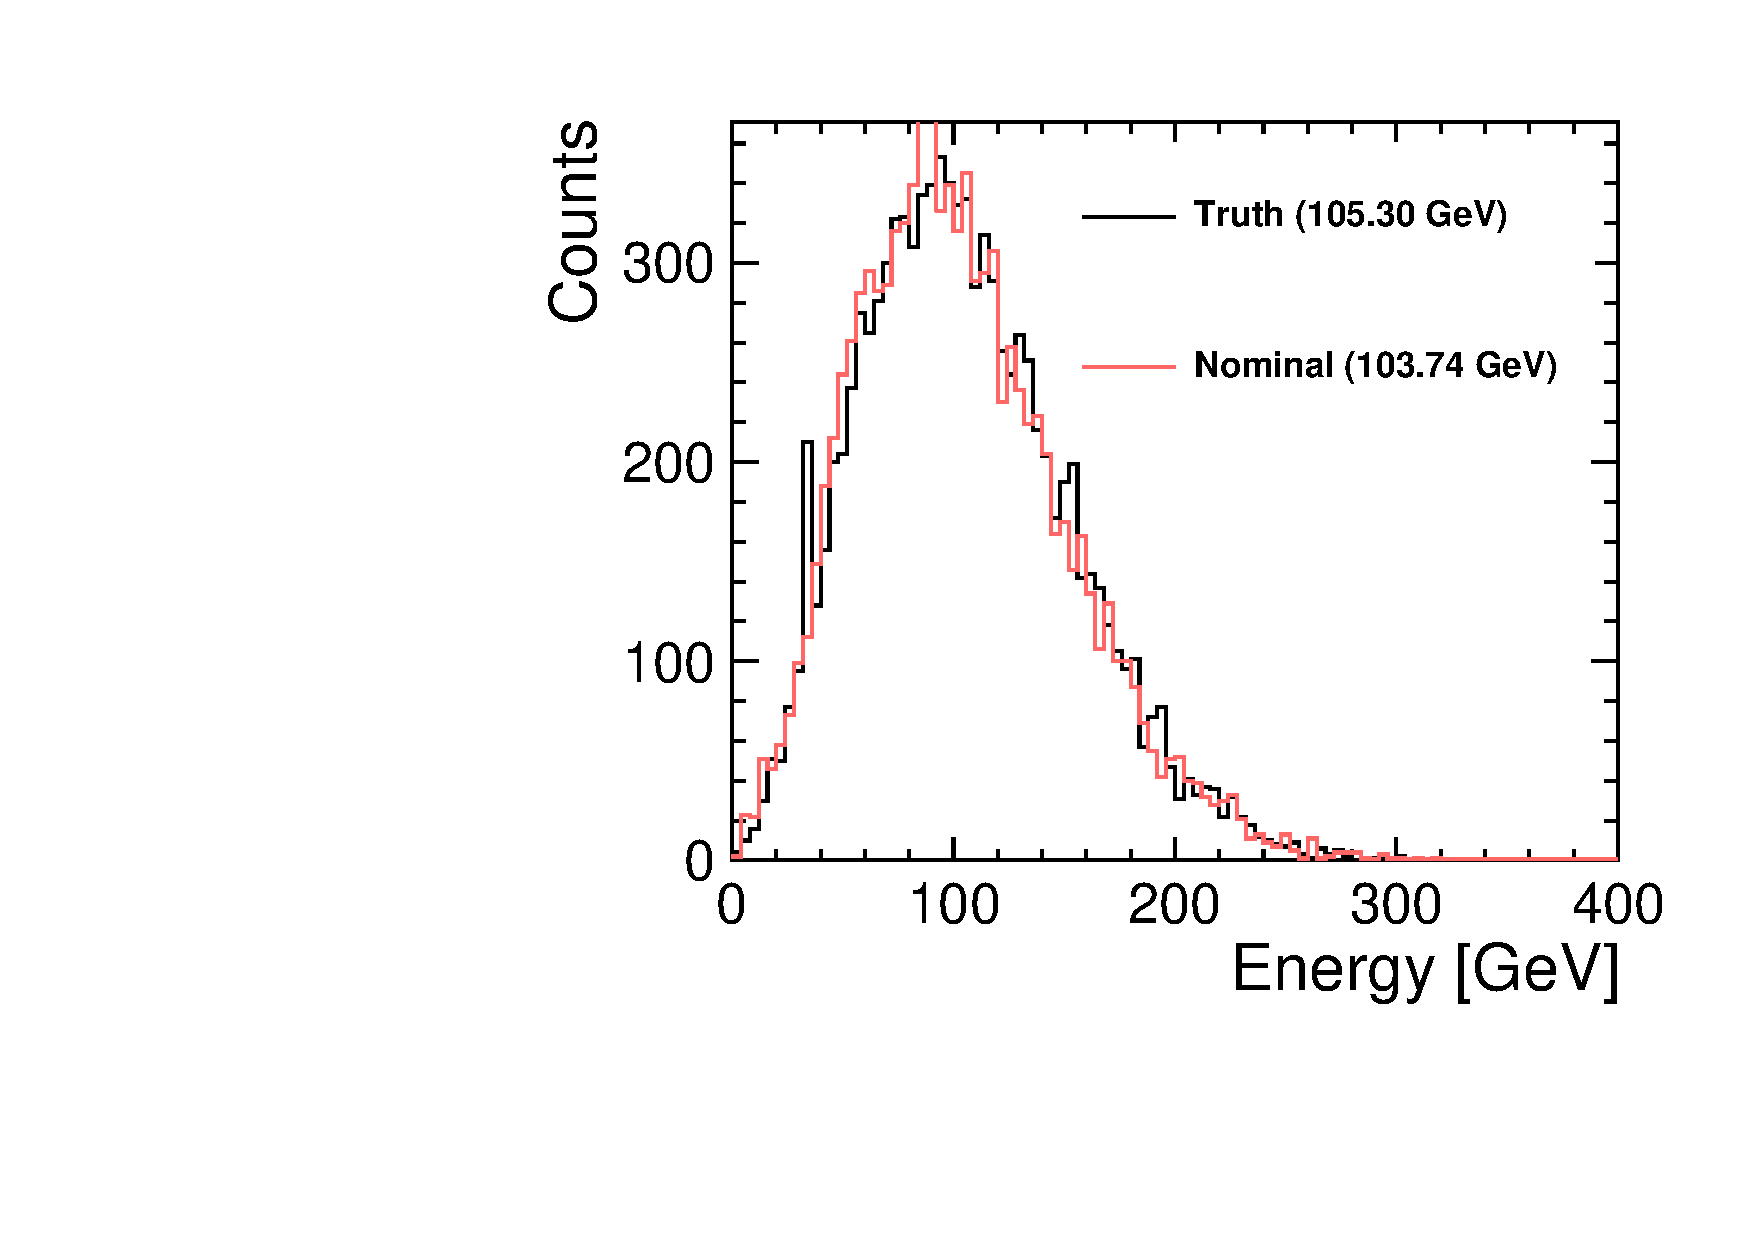
\includegraphics[width=5cm]{TrackClusterDistanceCut_Zuds380_photonEnergyRecoVsTruth.pdf}};
 
   \node[inner sep=0pt] (tmp) at (\xRefPosOne+3,\yRefPosOne-2.7)
    {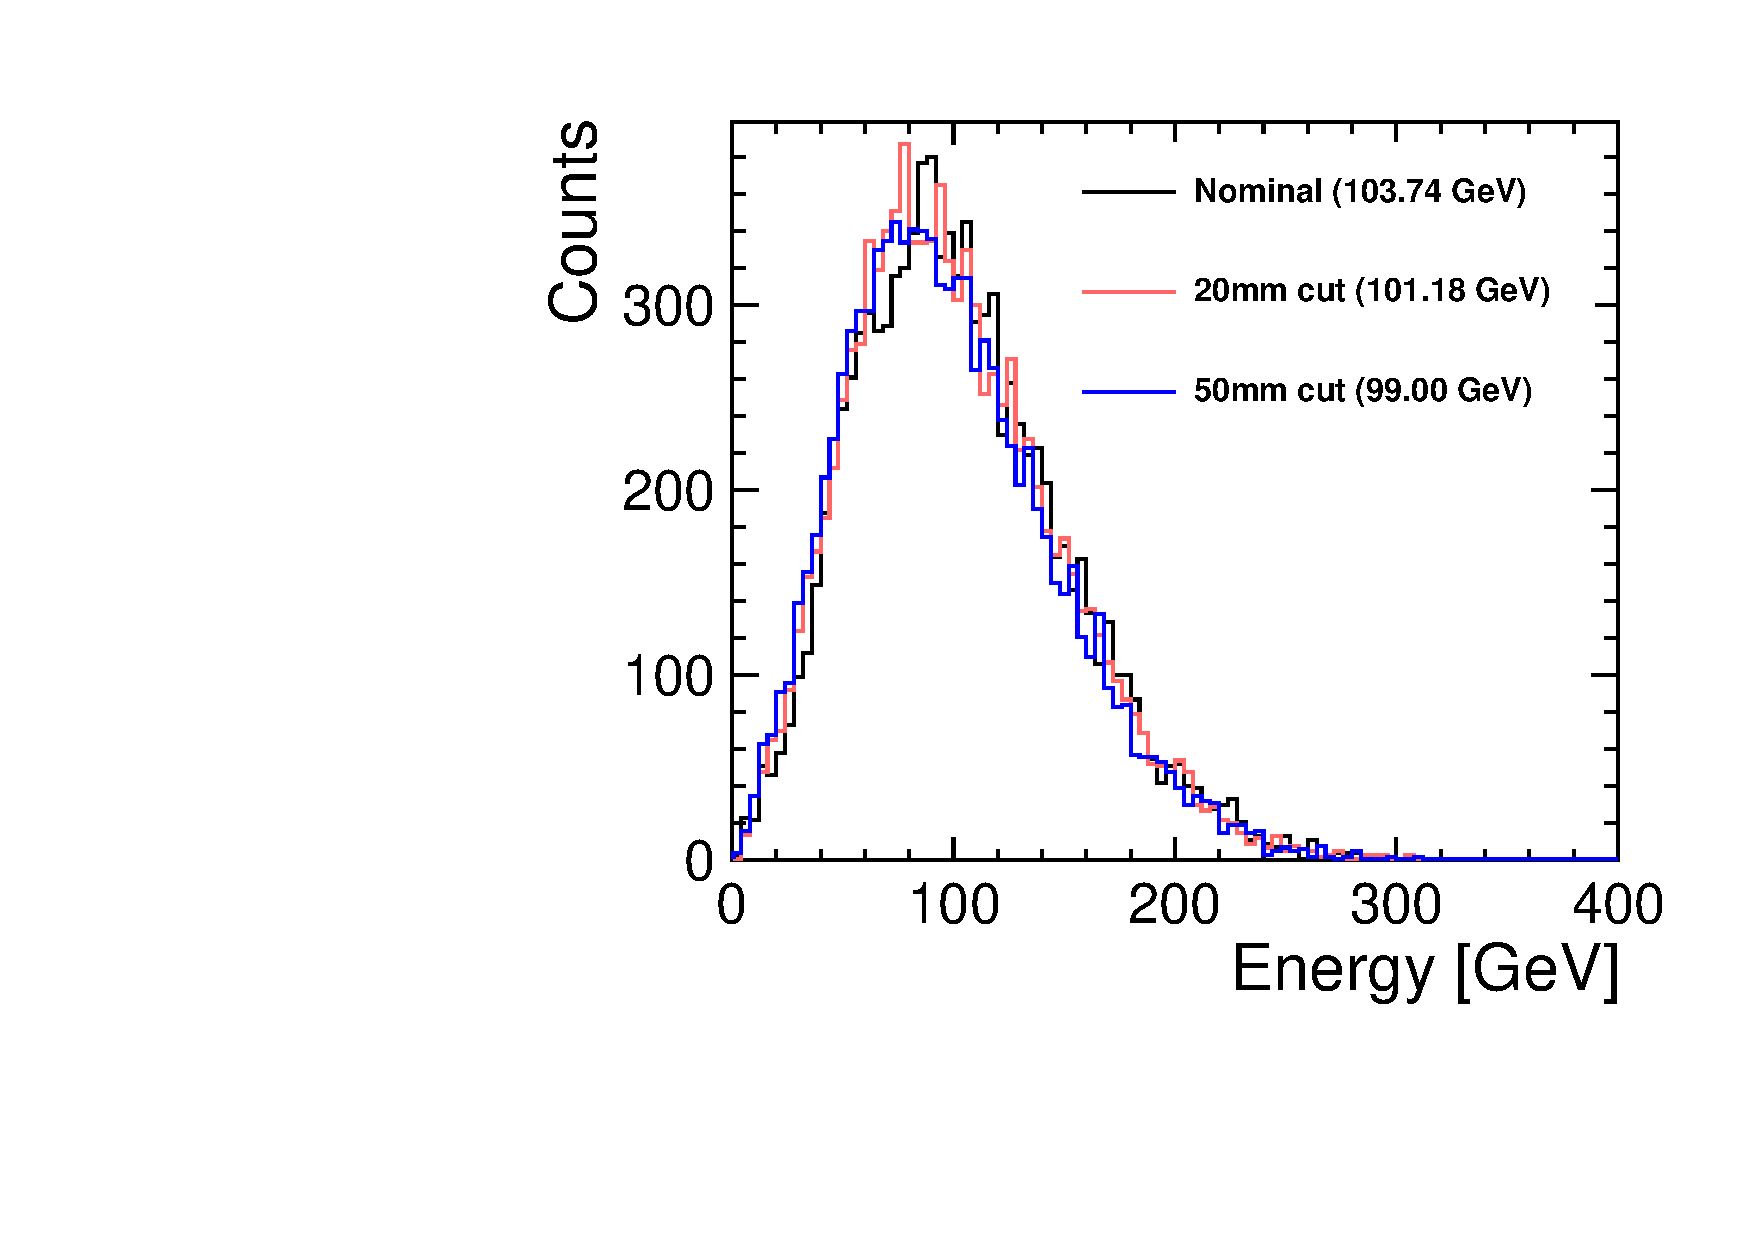
\includegraphics[width=5cm]{TrackClusterDistanceCut_Zuds380_photonRecoEnergy.pdf}};

\end{tikzpicture}
\end{frame}
%*****************************************************************************

%*****************************************************************************
\begin{frame}{\large \large Tracks Energy: 91 GeV (top) and 380 Zuds (bottom)}
 
\renewcommand{\yRefPosOne}{0}
\renewcommand{\xRefPosOne}{5.3}
\renewcommand{\xRefIncrementOne}{5.5}
\begin{tikzpicture}[overlay]

   \node[inner sep=0pt] (tmp) at (\xRefPosOne-3,\yRefPosOne+1.5)
    {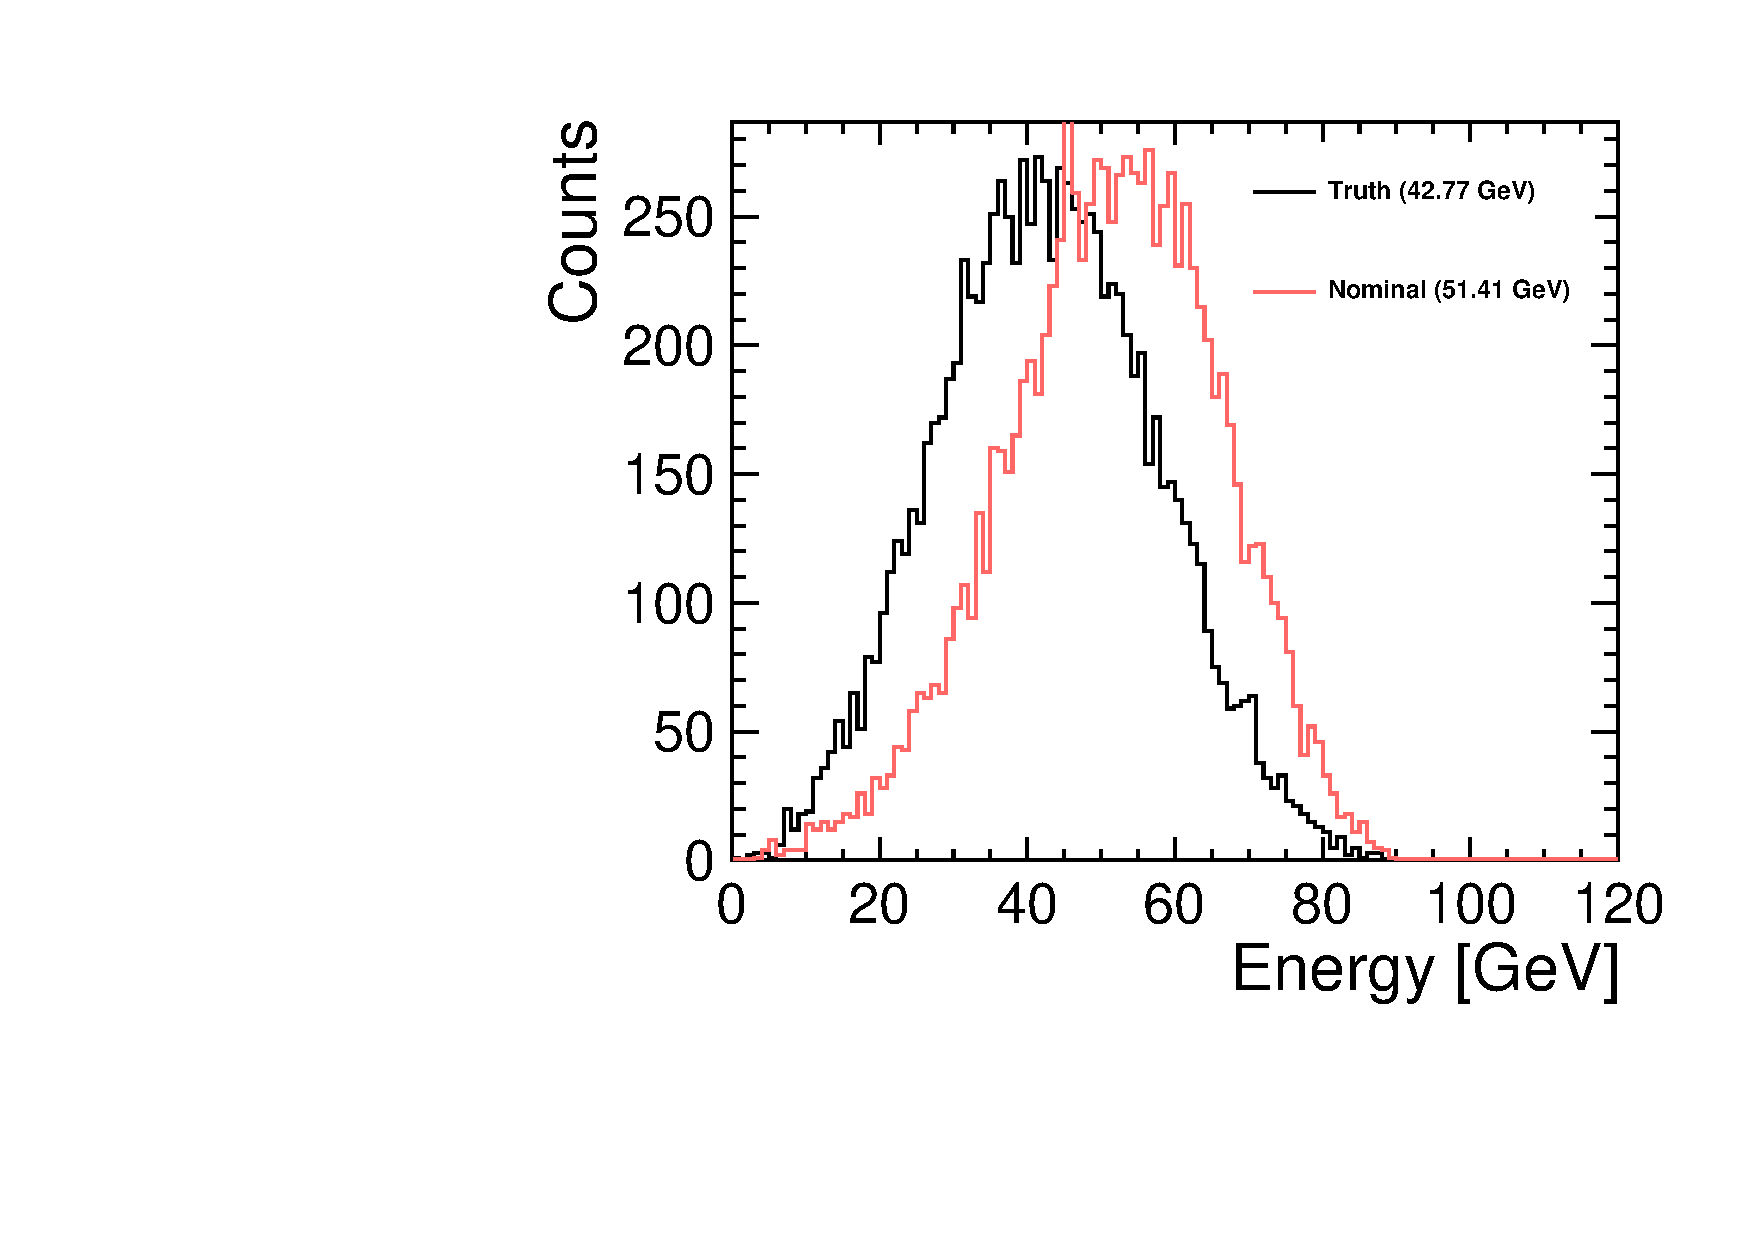
\includegraphics[width=5cm]{TrackClusterDistanceCut_Zuds91_tracksEnergyRecoVsTruth.pdf}};
 
   \node[inner sep=0pt] (tmp) at (\xRefPosOne+3,\yRefPosOne+1.5)
    {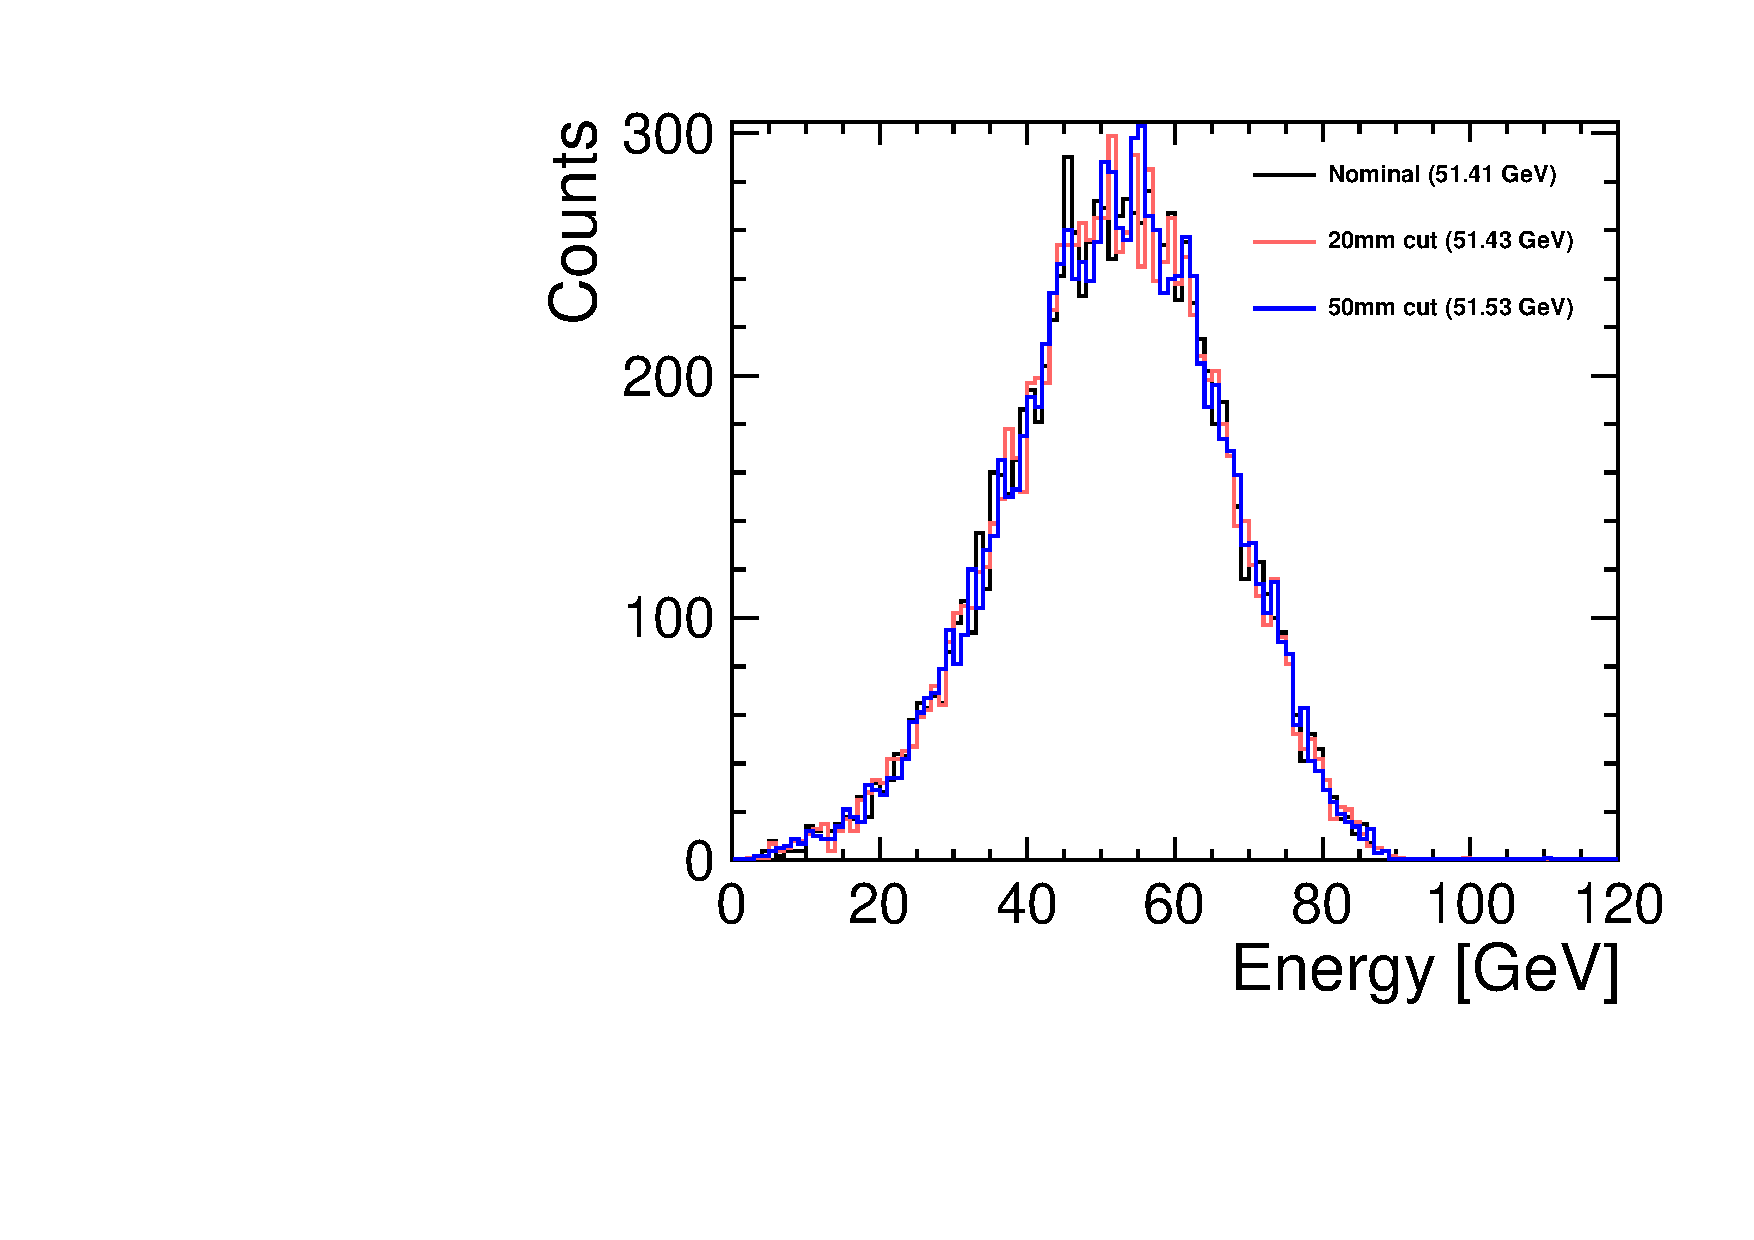
\includegraphics[width=5cm]{TrackClusterDistanceCut_Zuds91_tracksRecoEnergy.pdf}};
  
   \node[inner sep=0pt] (tmp) at (\xRefPosOne-3,\yRefPosOne-2.7)
    {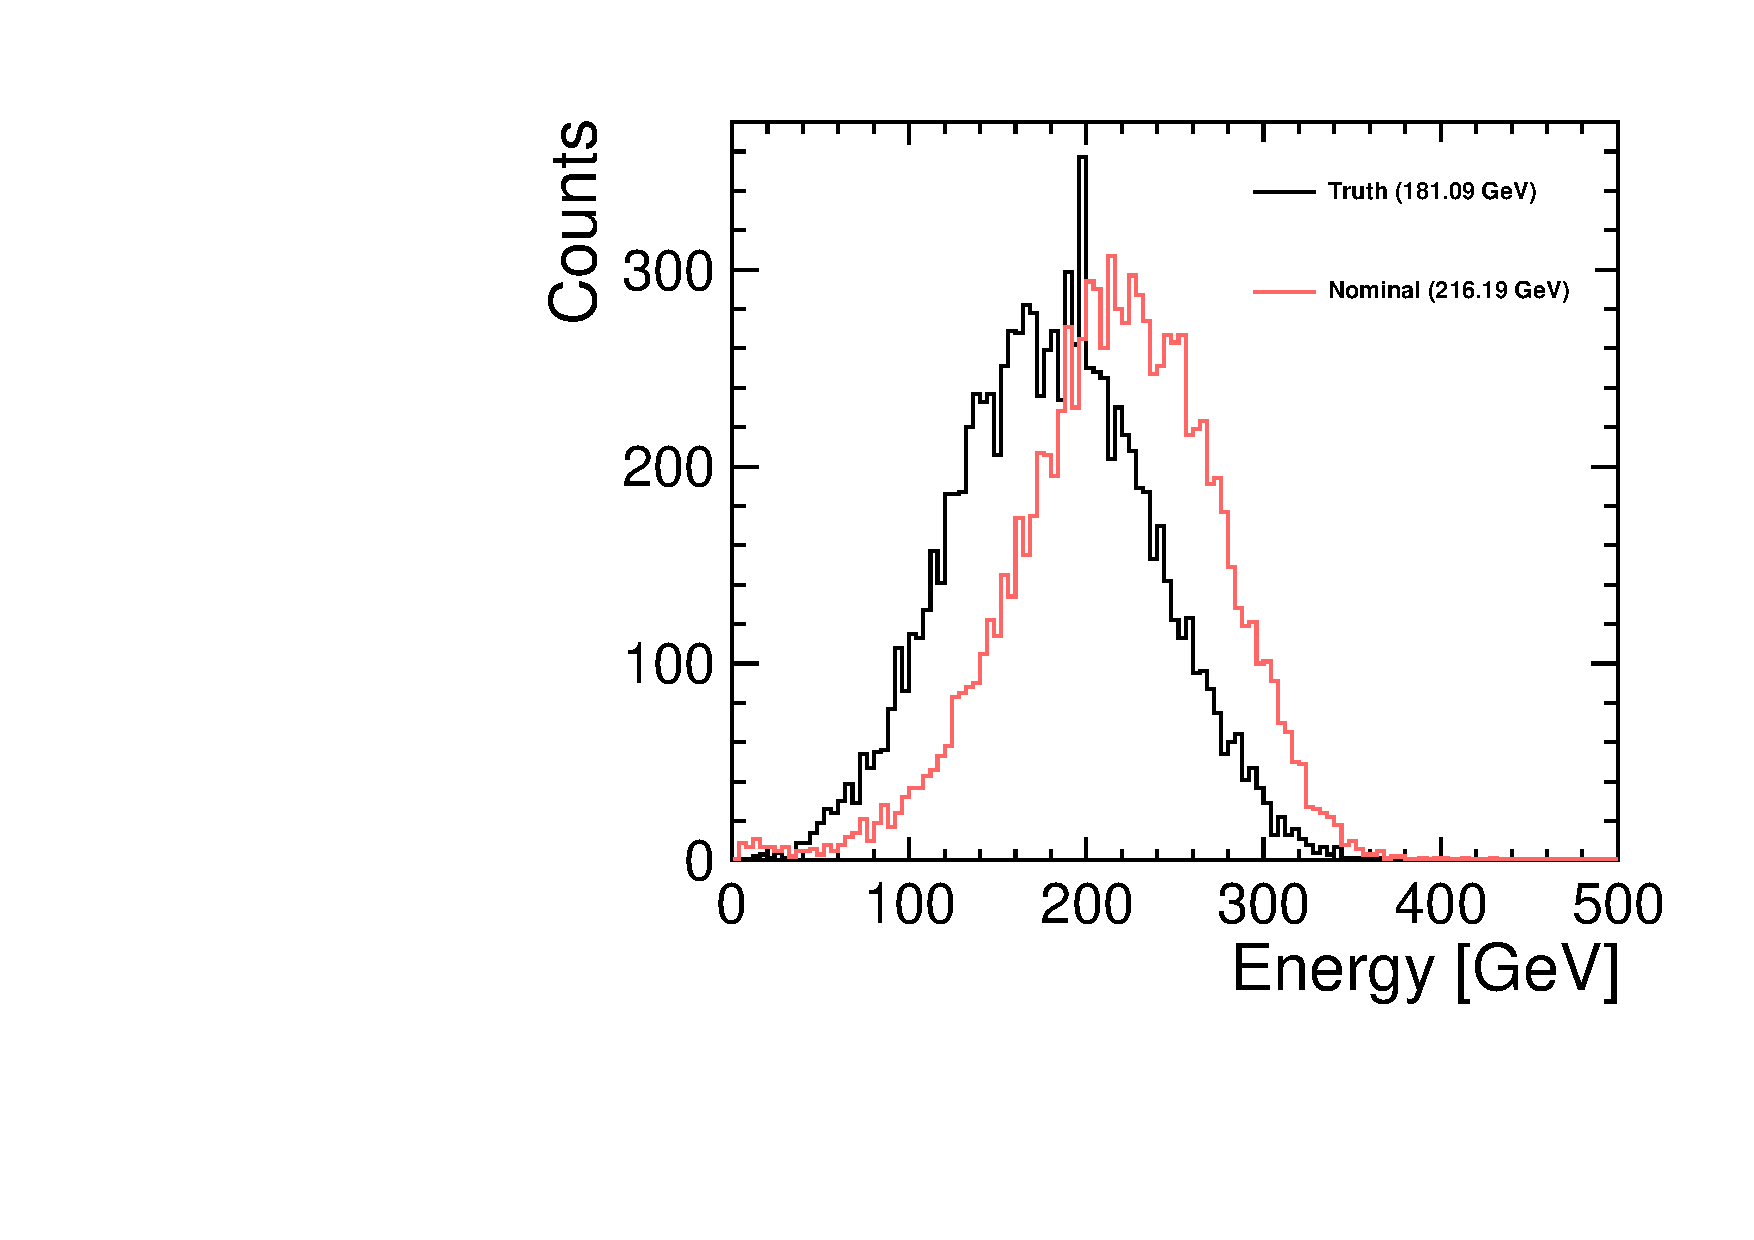
\includegraphics[width=5cm]{TrackClusterDistanceCut_Zuds380_tracksEnergyRecoVsTruth.pdf}};
 
   \node[inner sep=0pt] (tmp) at (\xRefPosOne+3,\yRefPosOne-2.7)
    {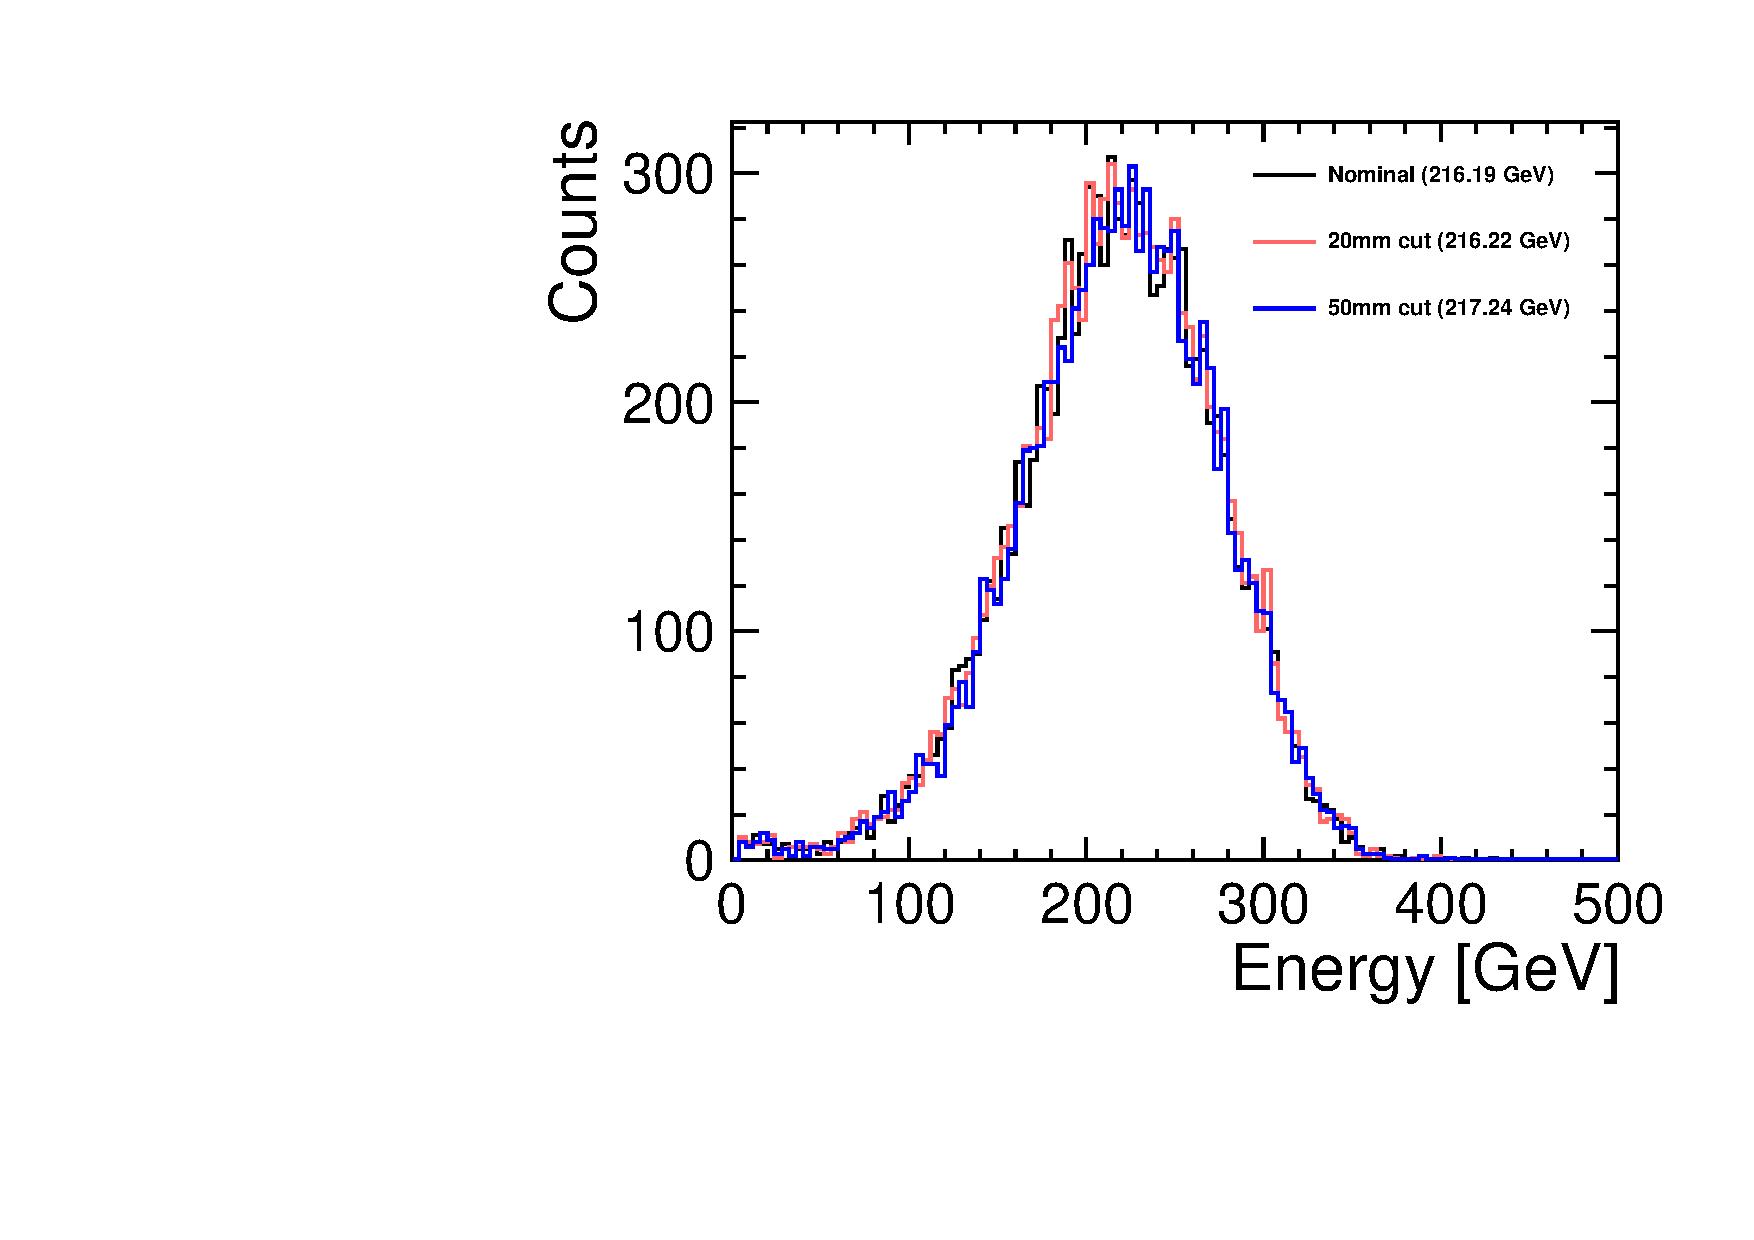
\includegraphics[width=5cm]{TrackClusterDistanceCut_Zuds380_tracksRecoEnergy.pdf}};

\end{tikzpicture}
\end{frame}
%*****************************************************************************

%*****************************************************************************
\begin{frame}{\large \large Neutral Hadrons Energy: 91 GeV (top) and 380 Zuds (bottom)}
 
\renewcommand{\yRefPosOne}{0}
\renewcommand{\xRefPosOne}{5.3}
\renewcommand{\xRefIncrementOne}{5.5}
\begin{tikzpicture}[overlay]

   \node[inner sep=0pt] (tmp) at (\xRefPosOne-3,\yRefPosOne+1.5)
    {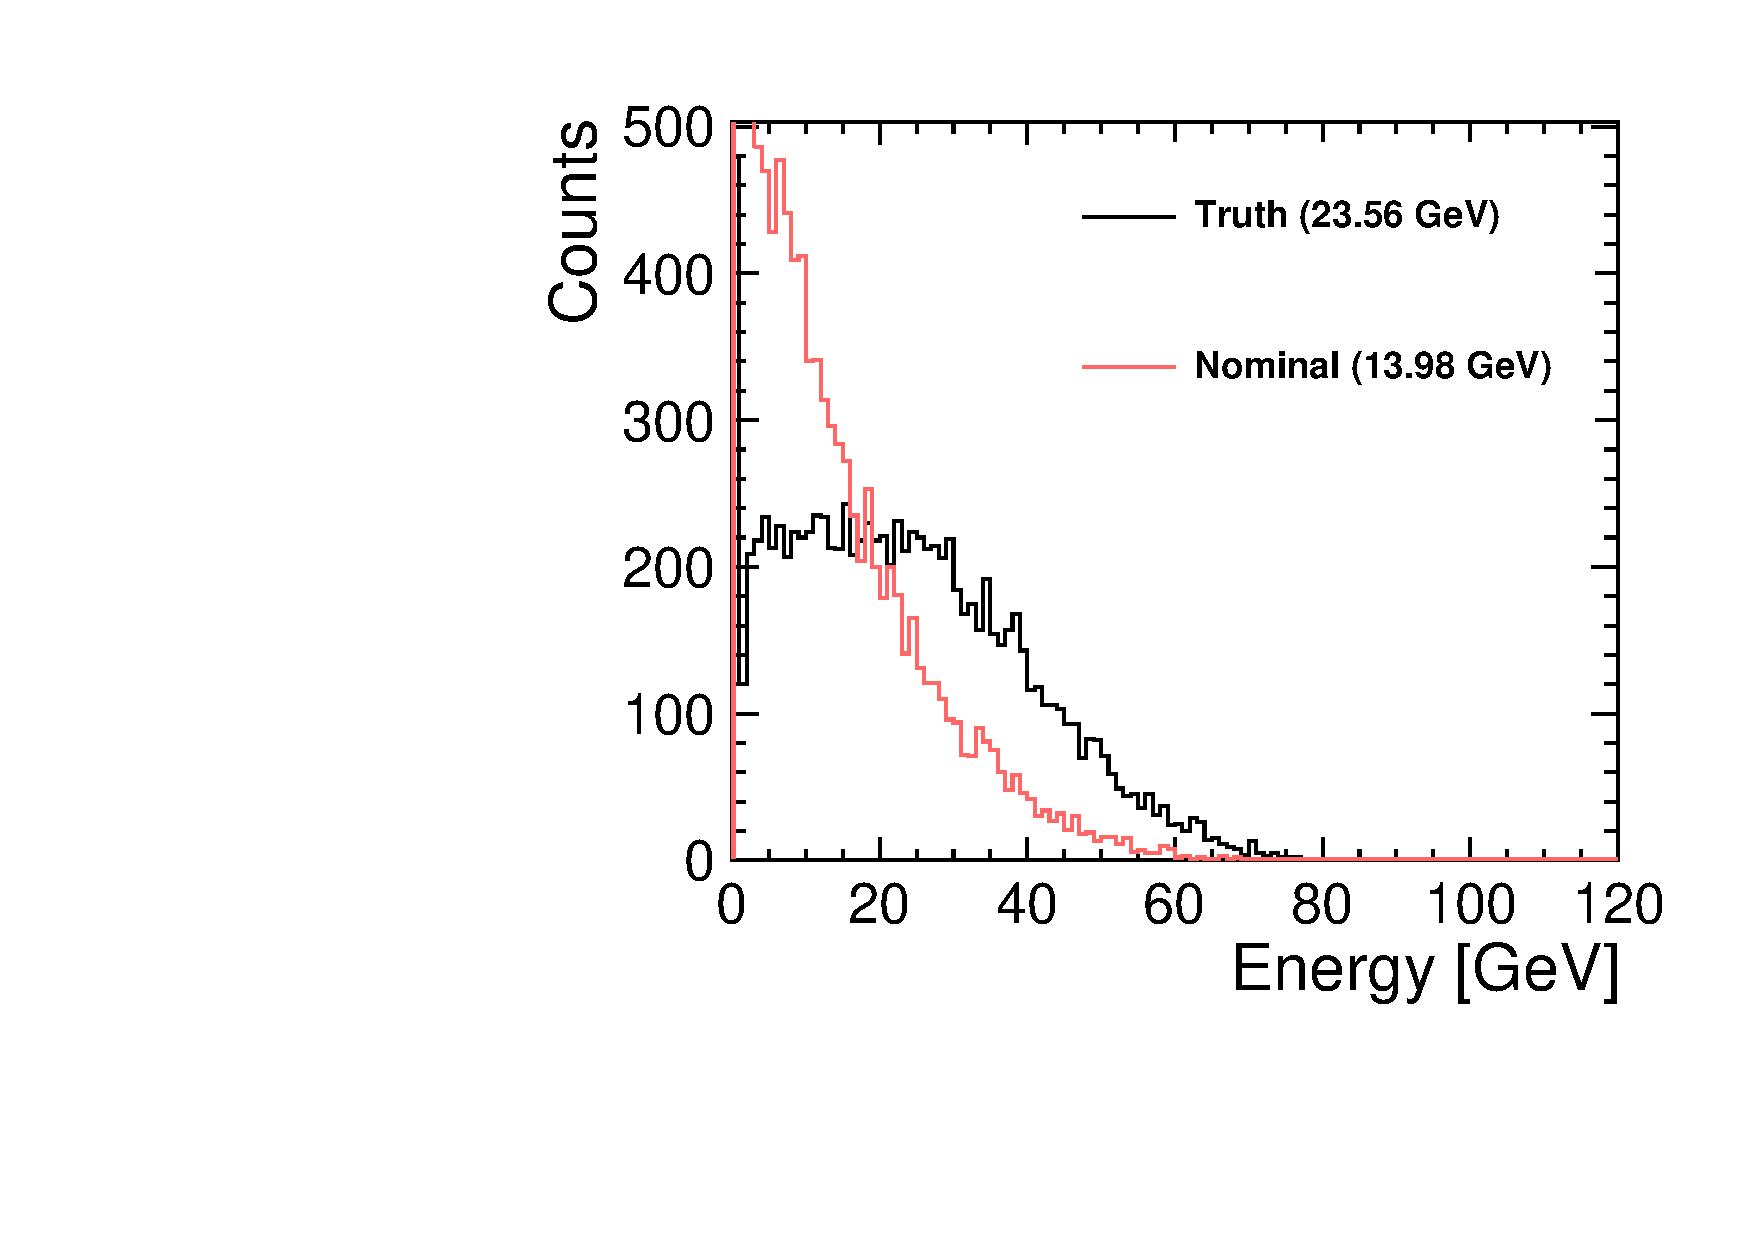
\includegraphics[width=5cm]{TrackClusterDistanceCut_Zuds91_neutralEnergyRecoVsTruth.pdf}};
 
   \node[inner sep=0pt] (tmp) at (\xRefPosOne+3,\yRefPosOne+1.5)
    {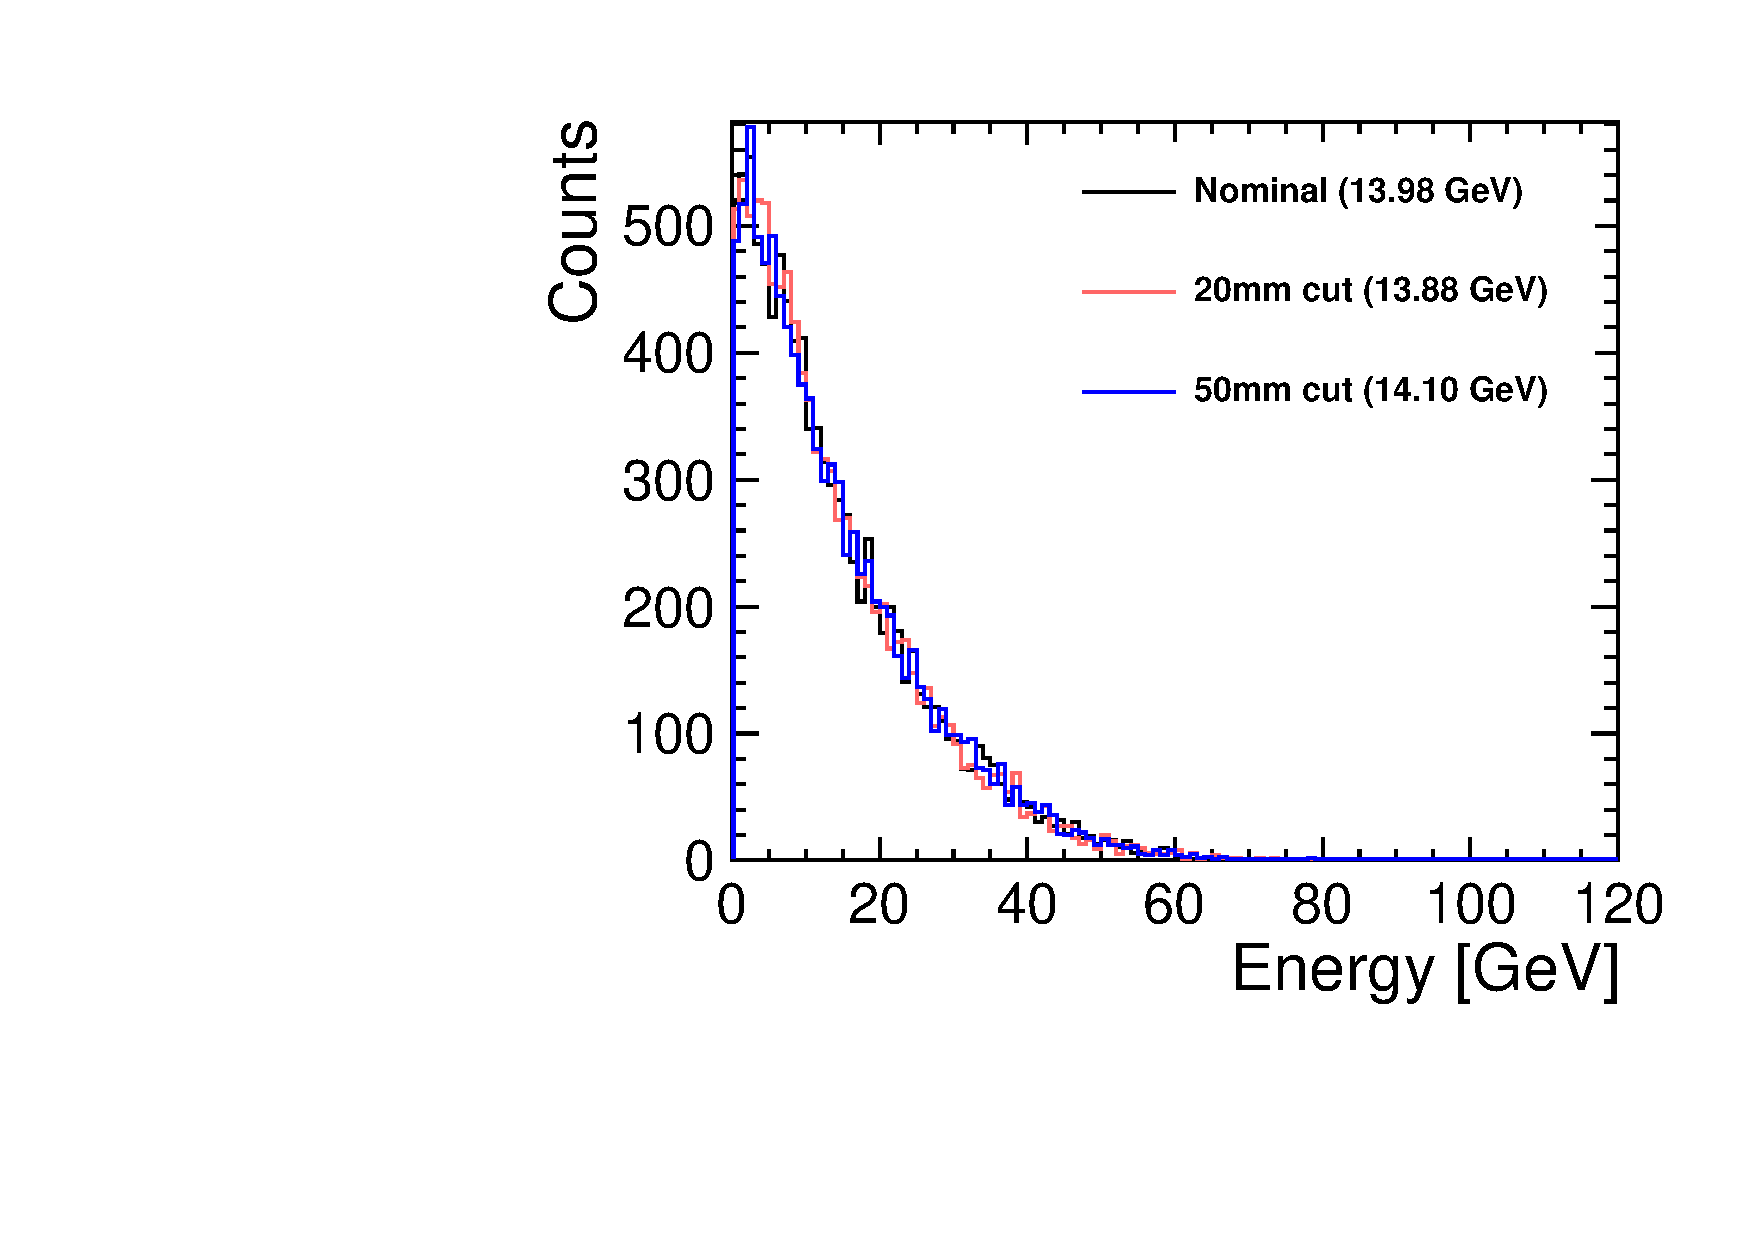
\includegraphics[width=5cm]{TrackClusterDistanceCut_Zuds91_neutralRecoEnergy.pdf}};
  
   \node[inner sep=0pt] (tmp) at (\xRefPosOne-3,\yRefPosOne-2.7)
    {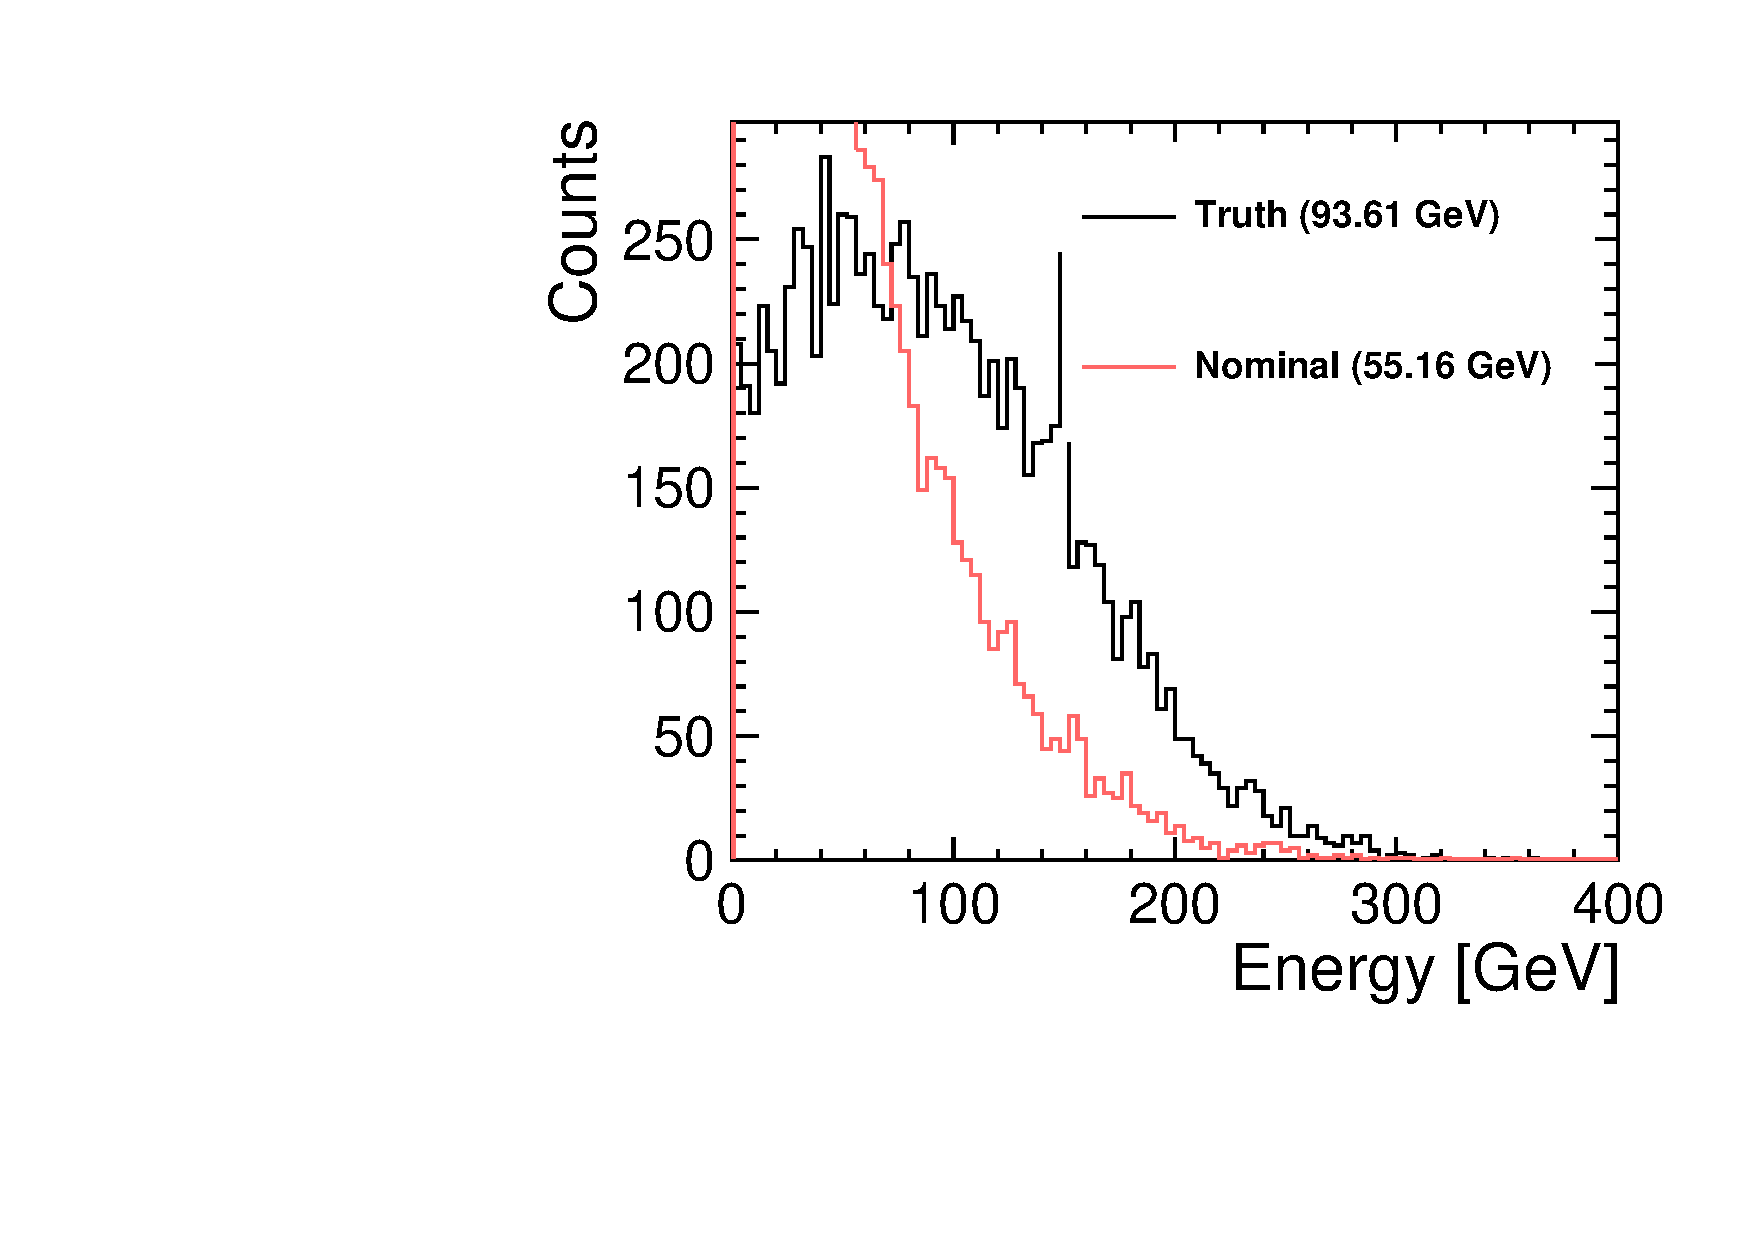
\includegraphics[width=5cm]{TrackClusterDistanceCut_Zuds380_neutralEnergyRecoVsTruth.pdf}};
 
   \node[inner sep=0pt] (tmp) at (\xRefPosOne+3,\yRefPosOne-2.7)
    {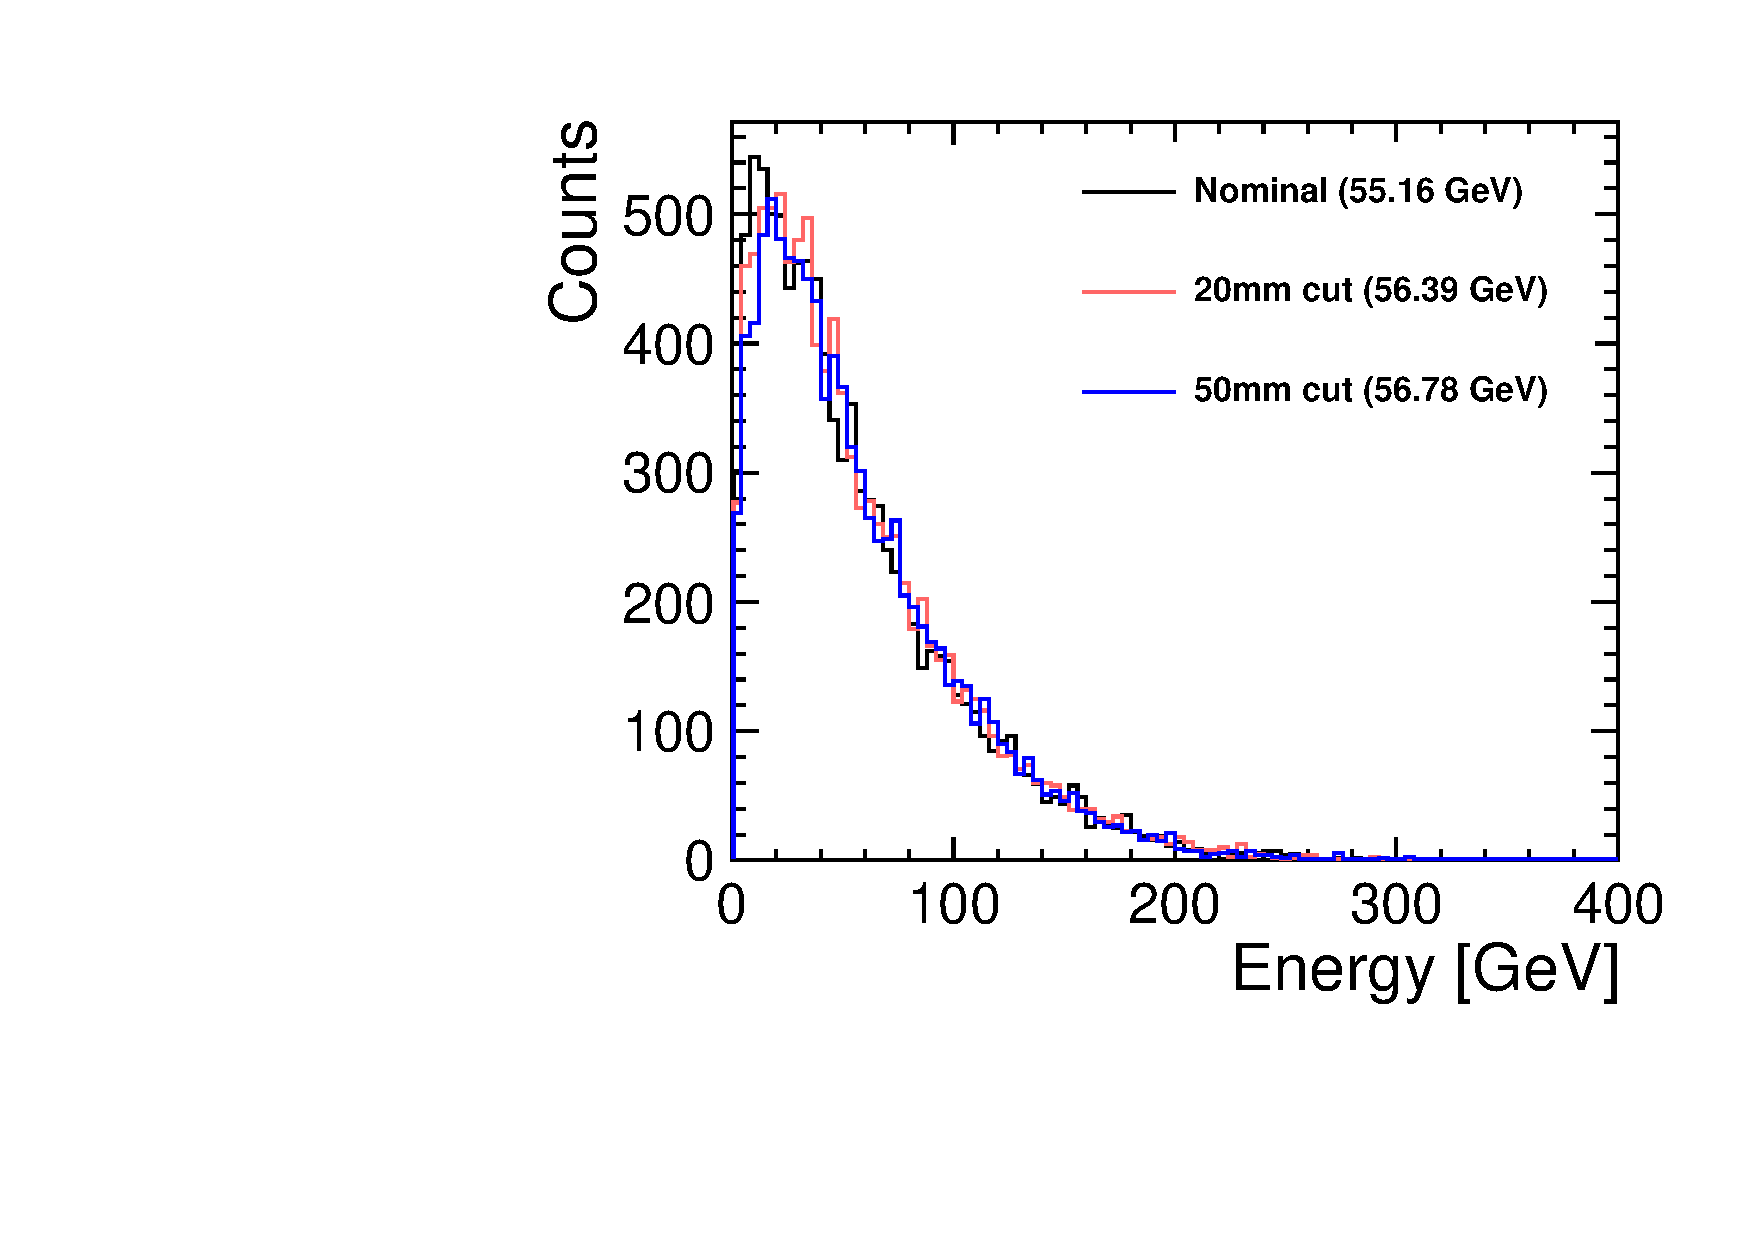
\includegraphics[width=5cm]{TrackClusterDistanceCut_Zuds380_neutralRecoEnergy.pdf}};

\end{tikzpicture}
\end{frame}
%*****************************************************************************

\end{document}

